\documentclass[a4paper,11pt]{article}
\usepackage[utf8]{inputenc}
\usepackage[T1]{fontenc}
\usepackage{graphicx}
\usepackage[T2A]{fontenc}
\usepackage[utf8]{inputenc}
\usepackage[english]{babel}
\usepackage{extsizes}
\usepackage{indentfirst}
\usepackage{fancyhdr}
\usepackage{geometry}
\usepackage{amsthm}
\usepackage{amsfonts}
\usepackage{mathtools}
\usepackage{graphicx}
\usepackage{wrapfig}
\usepackage{caption}
\usepackage{amssymb}
\usepackage{booktabs}
\usepackage{dsfont}
\usepackage[toc,page]{appendix}
\usepackage[export]{adjustbox}
\usepackage[percent]{overpic}
\usepackage[toc,page]{appendix}

% Default fixed font does not support bold face
\DeclareFixedFont{\ttb}{T1}{txtt}{bx}{n}{12} % for bold
\DeclareFixedFont{\ttm}{T1}{txtt}{m}{n}{12}  % for normal

% Custom colors
\usepackage{color}
\definecolor{deepblue}{rgb}{0,0,0.5}
\definecolor{deepred}{rgb}{0.6,0,0}
\definecolor{deepgreen}{rgb}{0,0.5,0}
\usepackage{listings}

% Python style for highlighting
\newcommand\pythonstyle{\lstset{
		language=Python,
		basicstyle=\ttm,
		otherkeywords={self},             % Add keywords here
		keywordstyle=\ttb\color{deepblue},
		emph={MyClass,__init__},          % Custom highlighting
		emphstyle=\ttb\color{deepred},    % Custom highlighting style
		stringstyle=\color{deepgreen},
		frame=tb,                         % Any extra options here
		showstringspaces=false            % 
	}}
	
	
	% Python environment
	\lstnewenvironment{python}[1][]
	{
		\pythonstyle
		\lstset{#1}
	}
	{}
	
	% Python for external files
	\newcommand\pythonexternal[2][]{{
			\pythonstyle
			\lstinputlisting[#1]{#2}}}
	
	% Python for inline
	\newcommand\pythoninline[1]{{\pythonstyle\lstinline!#1!}}

\theoremstyle{plain}
\newtheorem{thm}{Theorem}[part]% reset theorem numbering for each part
\newtheorem{lmm}[thm]{Lemma}
\newtheorem{crlr}[thm]{Corollary}

\theoremstyle{definition}
\newtheorem{defn}[thm]{Definition}
\newtheorem{exmp}[thm]{Example}
\newtheorem{rmrk}[thm]{Remark}
\newtheorem{asmp}[thm]{Assumptions}
\newtheorem{prps}[thm]{Proposition}
\newtheorem{cond}[thm]{Conditions}

\renewcommand{\theenumi}{\roman{enumi}}
\renewcommand{\labelenumi}{(\theenumi)}
\renewcommand\thepart{\arabic{part}}

\newcommand{\ME}{\mathbb{E}}
\newcommand{\MR}{\mathbb{R}}
\newcommand{\MP}{\mathbb{P}}
\newcommand{\MN}{\mathbb{N}}
\newcommand{\Var}{\operatorname{Var}}
\newcommand{\Cov}{\operatornamerm{Cov}}
\newcommand{\diag}{\operatorname{diag}}
\newcommand{\tr}{\operatorname{tr}}
\newcommand{\convdistr}{\xrightarrow{\mathcal{L}}}
\newcommand{\convprob}{\xrightarrow{\MP}}
\newcommand{\define}[1]{\textit{\textbf{#1}}}

\title{On the estimation of spectral distribution of integrated covariance matrices of high dimensional stochastic processes}
\author{Aleksandr Samarin}
\date{August 2017}

\begin{document}
	\maketitle
	
	In the 1-subject Master's program in Financial Mathematics of the Faculty of Mathematics and Natural Sciences of the CAU in Kiel
	
	presented by Aleksandr Samarin
	
	First referee:
	Second referee:
	Kiel, August 2017
	
	\pagebreak
	\begin{abstract}
		
		(COPIED FROM THE PAPER) \\
		We consider the estimation of integrated covariance (ICV) matrices
		of high dimensional diffusion processes based on high frequency
		observations. We start by studying the most commonly used estimator,
		the realized covariance (RCV) matrix. We show that in the
		high dimensional case when the dimension p and the observation frequency
		n grow in the same rate, the limiting spectral distribution
		(LSD) of RCV depends on the covolatility process not only through
		the targeting ICV, but also on how the covolatility process varies in
		time. We establish a Marcenko–Pastur type theorem for weighted
		sample covariance matrices, based on which we obtain a Marcenko–
		Pastur type theorem for RCV for a class C of diffusion processes.
		The results explicitly demonstrate how the time variability of the
		covolatility process affects the LSD of RCV. We further propose
		an alternative estimator, the time-variation adjusted realized covariance
		(TVARCV) matrix. We show that for processes in class C, the
		TVARCV possesses the desirable property that its LSD depends
		solely on that of the targeting ICV through the Marcenko–Pastur
		equation, and hence, in particular, the TVARCV can be used to recover
		the empirical spectral distribution of the ICV by using existing
		algorithms
	\end{abstract}
	
	\pagebreak
	\tableofcontents
	
	\pagebreak
	\part{Introduction}
	
	\section*{Motivation}
	\begin{rmrk}
		Diffusion processes are widely used to model financial asset price processes. For example, suppose that we have multiple stocks, say, $p$ stocks, whose price processes are denoted by $S_j(t)$ and $X_j(t) := \log S_j(t)$ for $j = 1, \dots, p$. Let
		\[ \mathbf{X}(t) = \big(X_1(t), \dots, X_p(t)\big)^T. \]
		Then a widely used model for $\mathbf{X}_t$ is
		\begin{equation} \label{X diffeq}
		d\mathbf{X}(t) = \boldsymbol{\mu}(t) dt + \Theta(t) d\mathbf{W}(t),
		\end{equation}
		where 
		\begin{itemize}
			\item $\boldsymbol{\mu}(t) = (\mu_1(t), \dots, \mu_p(t))^T$ is a $p$-dimensional drift process,
			\item $\Theta(t)$ -- $p \times p$ \define{covolatility process},
			\item $\mathbf{W}(t)$ -- $p$-dimensional standard Brownian motion.
		\end{itemize}
		If $\Theta(t) = \sigma(t) \cdot \mathbb{I}_{p \times p} $, we are in the case when all price processes are independent of each other and we can study them separately. In practice price on one good strongly depends on the price of the other. In this paper we consider special class of possibly dependent processes, which interrelation stays stable in time.
	\end{rmrk}


	\begin{defn} \
		\begin{enumerate}
			\item The \define{integrated covariance matrix (ICV)} is defined as follows
			\[\Sigma_p := \int_0^1\Theta(t) \cdot \Theta^T(t) dt.\]
			For $p=1$ ICV is called \define{integrated volatility}.
			\item Assume that we can observe the processes $X_j(t)$ at high frequency synchronously, say at time points $ \{\tau_\ell\}_{0 \leq \ell \leq n}$:
			\[ X_j(\tau_\ell) = \log S_j(\tau_\ell), \quad \ell = 0, 1, \dots, n, j = 1, \dots, p. \]
			 Then \define{realized covariance matrix (RCV)} is
			\begin{equation} \label{RCV}
				\Sigma_p^{RCV} := \sum_{\ell=1}^{n}\Delta \mathbf{X}_\ell(\Delta \mathbf{X}_\ell)^T,
			\end{equation}
			where 
			\[ \Delta \mathbf{X}_\ell :=
			\begin{pmatrix}
			\Delta {X_1}_\ell \\
			\vdots \\
			\Delta {X_p}_\ell
			\end{pmatrix}
			=
			\begin{pmatrix}
			X_1(\tau_{\ell}) - X_1(\tau_{\ell-1}) \\
			\vdots \\
			X_p(\tau_{\ell}) - X_p(\tau_{\ell-1})
			\end{pmatrix}. \]
			For $p=1$ RCV is called \define{realized volatility}.
		\end{enumerate}
	\end{defn}
	
	\begin{exmp} \label{exmp X3}
	    Let's take $p = 3$, zero drift $\boldsymbol{\mu}(t) = (0, 0, 0)^T$ and 
		\[ \Theta(t) = \begin{pmatrix}
		1 & \cos(\pi t) & \sin (\pi t) \\
		\cos(\pi t) & 1 & 0 \\
		\sin (\pi t) & 0 & 1
		\end{pmatrix}. \]
		Then our process satisfies
		\[ d\mathbf{X}(t) = \begin{pmatrix}
		dW_1(t)+\cos(\pi t) dW_2(t) +\sin(\pi t)dW_3(t)  \\
	    \cos(\pi t) dW_1(t) + dW_2(t) \\
		\sin(\pi t) dW_1(t)+ dW_3(t)
		\end{pmatrix}. \]
		We have
		\[ \Theta(t) \cdot \Theta^T(t) = \begin{pmatrix}
		2 & 2\cos(\pi t) & 2\sin (\pi t) \\
		2\cos(\pi t) & \cos^2(\pi t) + 1 & \cos(\pi t)\sin(\pi t) \\
		2\sin (\pi t) & \cos(\pi t)\sin(\pi t) & \sin^2(\pi t)+1
		\end{pmatrix} \]
		and corresponding ICV matrix is
		\[ \Sigma_3 = \begin{pmatrix}
		2 & 0 & \frac{4}{\pi} \\
		0 & \frac{3}{2} & 0 \\
		\frac{4}{\pi} & 0 & \frac{3}{2}
		\end{pmatrix}. \]
	\end{exmp}
	
	\begin{rmrk} \
		\begin{enumerate}
			\item 
			Intuitively, one can wish zero elements of the ICV matrix to show the independence of one process from another. But in Example \ref{exmp X3}, where all the processes are related with each other in some sense, we still have zero values in $\Sigma_3$. It should be noted that if $\mathbf{X}(t)$ is a vector of log-price processes, then over short time period, say, one day, it is reasonable to assume that the correlation structure doesn't change.
			\item One of the major problems in most of the models, based on the theory of stochastic calculus and applied to financial markets, is the estimation of true covariance. In our case the final goal is to find an estimator of an ICV matrix. In the next section we show how RCV matrix does the job.
		\end{enumerate}
	\end{rmrk}
	
	\begin{figure}
		\begin{center} \centering
			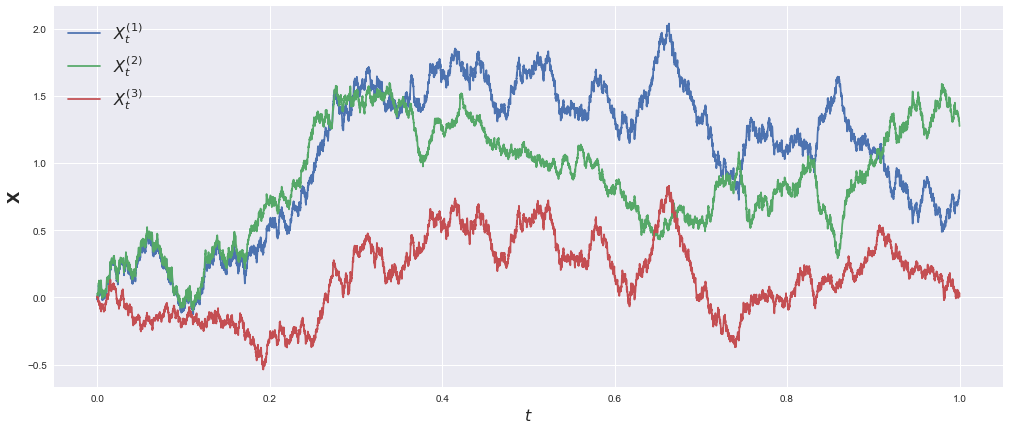
\includegraphics[scale=0.4]{X3}
			\caption{$\mathbf{X}(t)$ from Example \ref{exmp X3}}
			\smallskip
			\small
			One can observe that $X_1(t)$ and $X_2(t)$ have strong positive correlation in the beginning, which decreases over time and later, when $t$ approaches $1$, turns into negative one. Meanwhile $X_3(t)$ has independent fluctuations on the borders, but in the middle it repeats the behavior of $X_1(t)$.
		\end{center}
	\end{figure}
	
	\section*{The relation between RCV and ICV}
	
	\begin{defn} \label{stoch calc notions}
		Recall the basic notions from the theory of stochastic calculus (w.l.o.g. we assume that all the processes have a starting point at $0$ a.s.):
		\begin{enumerate}
			\item An \define{Itô process} $X(t)$ is defined to be an adapted stochastic process that can be expressed as the sum of an integral with respect to time and an integral with respect to Brownian motion:
			\[ X(t) = \int_{0}^{t} \mu(s) ds + \int_{0}^{t} \sigma(s) dW(s). \]
			\item Let $X$ be a continuous local martingale. Then $[X]_t$ with
			\[ [X](t) = X^2(t) - 2 \int_0^t X(s)dX(s) \]
			is called \define{quadratic variation} of $X$. Note that for deterministic processes quadratic variation is equal to $0$.
			\item The \define{quadratic covariation} of two continuous semimartingales $X$ and $Y$ is defined as follows:
			\[ [X, Y](t) = \frac{1}{4}([X + Y](t) - [X-Y](t)). \]
			\item Let $X$ and $Y$ be Itô processes with volatilities ${\sigma_X}(t)$ and ${\sigma_Y}(t)$ with respect to the same Brownian motion, then
			\[ [X, Y](t) = \int_0^t {\sigma_X}(s){\sigma_Y}(s) ds. \]
			\item Quadratic covariation is symmetric and bilinear map:
			\[ [X + Y, Z](t) = [X, Z](t) + [Y, Z](t), \]
			\[ [X, Y + Z](t) = [X, Y](t) + [X, Z](t), \]
			\[ [X, Y](t) = [Y, X](t), \quad [X](t) = [X, X](t). \]
		\end{enumerate}
	\end{defn}
	
	\begin{exmp} \label{quad var} \
		\begin{enumerate}
			\item 
			Let us first consider two-dimensional case with $\boldsymbol{\mu}(t) = (\mu_1(t), \mu_2(t))^T$ and
			\[\Theta(t) = \begin{pmatrix}
			\sigma_{11}(t) & \sigma_{12}(t) \\
			\sigma_{21}(t) & \sigma_{22}(t)
			\end{pmatrix} \]
			Then $\mathbf{X}(t) = (X(t), Y(t))^T$, where 
			\[X(t) = \int_0^t\mu_1(s) ds + \int_0^t\sigma_{11}(s) dW_1(s) + \int_0^t\sigma_{12}(s) dW_2(s)\] 
			and
			\[Y(t) = \int_0^t\mu_2(s) ds + \int_0^t\sigma_{21}(s) dW_1(s) + \int_0^t\sigma_{22}(s) dW_2(s).\]
			Using Definition \ref{stoch calc notions} we get
			\begin{equation}
			[X](t) = \int_{0}^{t}(\sigma_{11}^2(s) +\sigma_{12}^2(s)) ds, \quad  [Y](t) = \int_{0}^{t}(\sigma_{21}^2(s) +\sigma_{22}^2(s)) ds
			\end{equation}
			and
			\begin{equation} \label{quadratic variation Ito}
			[X, Y](t) = \int_{0}^{t}(\sigma_{11}(s)\sigma_{21}(s) + \sigma_{12}(s)\sigma_{22}(s)) ds. 
			\end{equation}
			Let us look at the quadratic covariation $[X, Y]$ at time $1$. It is defined as follows: let $\Pi = \{ \tau_0, \dots, \tau_n \}$ be a partition of $[0, 1]$ (i.e. $0 = \tau_0 < \tau_1 < \dots \tau_n = 1$) and set up the sampled cross variation
			\begin{equation} \label{cross variation}
			\sum_{\ell = 1}^{n} \Delta X_\ell \Delta Y_\ell = \sum_{\ell = 1}^{n} (X(\tau_\ell) - X(\tau_{\ell-1})) \cdot (Y(\tau_\ell) - Y(\tau_{\ell-1})).
			\end{equation}
			Now let the number of partition points $n$ go to infinity as the length of the longest subinterval $\| \Pi \| = \max_{1 \leq \ell \leq n}(\tau_{\ell} - \tau_{\ell-1}) $ goes to zero. The sum in \eqref{cross variation} converges in probability to $[X, Y](1)$. This limit is given by the right-hand side of \eqref{quadratic variation Ito}. This assertion follows from the standard theorems in the theory of stochastic calculus. Writing formally,
			\[  \lim_{n \rightarrow \infty} \sum_{\ell = 1}^{n} \Delta X_\ell \Delta Y_\ell \xrightarrow{\mathbb{P}} [X, Y](1). \]
			Hence,
			\[
			\lim_{n \rightarrow \infty} \sum_{\ell=1}^{n}\Delta \mathbf{X}_\ell(\Delta \mathbf{X}_\ell)^T
			= \lim_{n \rightarrow \infty} \sum_{\ell=1}^{n}\begin{pmatrix}
			(\Delta X_\ell)^2 & \Delta X_\ell \Delta Y_\ell \\
			\Delta Y_\ell \Delta X_\ell & (\Delta Y_\ell)^2
			\end{pmatrix} 
			\xrightarrow{\mathbb{P}} 
			\begin{pmatrix}
			[X](1) & [X, Y](1) \\
			[Y, X](1) & [Y](1)
		    \end{pmatrix}.
			\]
			On the other hand,
			\[ \Theta(t) \cdot \Theta^T(t) = \begin{pmatrix}
			\sigma_{11}^2(t) + \sigma_{12}^2(t) & \sigma_{11}(t)\sigma_{21}(t) + \sigma_{12}(t)\sigma_{22}(t) \\
			\sigma_{11}(t)\sigma_{21}(t) + \sigma_{12}(t)\sigma_{22}(t)  & \sigma_{21}^2(t) + \sigma_{22}^2(t)
			\end{pmatrix}. \]
			Taking the integral of $\Theta(t) \cdot \Theta^T(t)$ we conclude that
			\[ \lim_{n \rightarrow \infty} \Sigma_2^{RCV} \xrightarrow{\mathbb{P}} \Sigma_2. \]
			\item 
			The convergence of realized covariance to ICV can be generalized for arbitrary $p$. Let's set $\boldsymbol{\mu}(t) = (\mu_1(t), \dots, \mu_p(t))^T$ and
			\[ 
			\Theta(t) = \begin{pmatrix}
			\Theta_{11}(t) & \dots & \Theta_{1p}(t) \\
			\vdots & \ddots & \vdots \\
			\Theta_{p1}(t) & \dots & \Theta_{pp}(t)
			\end{pmatrix}.
			\]
			Then we have $\mathbf{X}(t) = (X_1(t), \dots, X_p(t))^T$ with
			\[X_j(t) =  \int_0^t\mu_j(s) ds +  \sum_{i=1}^{p} \int_0^t \Theta_{ji}(s) dW_i(s) \]			
			for all $1 \leq j \leq p$. By Definition \ref{stoch calc notions} again
			\[ [X_j](t)= \int_0^t \bigg( \sum_{i=1}^{p} \Theta_{ji}^2(s) \bigg) ds \]
			and
			\[ [X_j, X_k](t) = \int_0^t \bigg(  \sum_{i=1}^{p} \Theta_{ji}(s) \cdot \Theta_{ki}(s) \bigg) ds \]
			for all $1 \leq j,k \leq p$.
			We also have
			\[ 
			\Big(\Theta(t) \cdot \Theta^T(t) \Big)_{jk}   = \sum_{i=1}^{p} \Theta_{ji}(t) \cdot \Theta_{ki}(t).
			\]
			Therefore, we get
			\[  \lim_{n \rightarrow \infty} \sum_{\ell=1}^{n}\Delta \mathbf{X}_\ell(\Delta \mathbf{X}_\ell)^T \xrightarrow{\mathbb{P}} [\mathbf{X}, \mathbf{X}](1), \]
			where 
			\[ \Big( [\mathbf{X}, \mathbf{X}](t)\Big)_{ij} = [X_i, X_j](t), \]
			and finally
			\[ \lim_{n \rightarrow \infty} \Sigma_p^{RCV} \xrightarrow{\mathbb{P}} \Sigma_p. \]
		\end{enumerate}
		
		\begin{rmrk}
			Let ICV matrix $\Sigma_p$ be deterministic. RCV matrix $\Sigma_p^{RCV}$, on the other side, is random by definition. In Example \ref{quad var} we used quadratic covariation as an intermediate step to prove the convergence of one matrix to another. Alternatively to Definition \ref{stoch calc notions} (iii) quadratic covariation can be defined as a limit of the sum of squared differences, so it is also random. Having almost sure degenerate distribution of quadratic covariation is one of the major properties of Itô processes and it doesn't need to hold for all martingales in general.
		\end{rmrk}
		
	\end{exmp}
	
	\pagebreak
	\part{Marchenko-Pastur law}
	\section*{Empirical spectral distribution}
	\begin{rmrk}
		In Remark \ref{quad var} we claimed the convergence of RCV matrix to ICV for any finite $p$. In practice, however, it might be the case that the number of processes is approximately equal to the number of observations for each process. Theoretically, the problem arises when the dimension of $p$ has at least the same rate of growth as $n$. In this case the convergence is not well defined, because the RCV matrix has the unlimited size.
		Then, it is more convenient to study another criteria.
	\end{rmrk}
	
	\begin{defn}
		Let $\{\lambda_j:j=1,\dots, p\}$ be set of eigenvalues of matrix $A$, then
		\[F^{A}(x) := \frac{\#\{j:\lambda_j \leq x\}}{p}, \quad x \in \MR, \]
		is called \define{empirical spectral distribution (ESD)} of $A$.
	\end{defn}
	
	\begin{exmp} \label{ESD finite p}
		Take the simplest case with $\boldsymbol{\mu}(t) = 0$ and $\Theta(t) = \sigma \cdot \mathbb{I}_{p \times p}$ with some constant $\sigma$. Then $\Sigma_p = \sigma^2 \mathbb{I}_{p \times p}$ and its ESD
		\[ F^{\Sigma_p}(x) = 1_{[\sigma^2, \infty)}(x) \]
		is a simple step function. In general case, where $\Sigma_p$ have different eigenvalues, ESD is a combination of such step functions.
	\end{exmp}
	
	\begin{rmrk}
		A naive estimator of the spectral distribution of the ICV matrix $\Sigma_p$ is the spectral distribution of the RCV matrix $\Sigma_p^{RCV}$. In particular, one might wish that the ESD $F^{\Sigma_p^{RCV}}$ of $\Sigma_p^{RCV}$ would approximate $F^{\Sigma_p}$ well when the value of $n$ sufficiently high, namely
		\[ \lim_{n \rightarrow \infty} F^{\Sigma_p^{RCV}} \rightarrow F^{\Sigma_p}. \]
		From the large dimensional random matrix theory (LDRMT), we now understand quite well that in the high dimensional setting this good wish won't always come true. For example, in the simplest case when the drift process $\boldsymbol{\mu}(t)$ is $0$, covolatility process $\Theta(t)$ is constant, and observation times $\tau_\ell$ are equally spaced ($\tau_\ell = \ell / n$), we are in the setting of estimating the usual covariance matrix using the sample covariance matrix, given $n$ i.i.d. $p$-dimensional observations $(\Delta \mathbf{X}_\ell)_{\ell=1, \dots, n}$. From LDRMT, we know that if $p/n$ converges to a non-zero number and the ESD $F^{\Sigma_p}$ of the true covariance matrix converges, then the ESD $F^{\Sigma_p^{RCV}}$ of the sample covariance matrix also converges (see e.g. Marchenko and Pastur (1967), Yin(1968), Silverstein and Bai (1995) and Silverstein(1995)). However, the relationship between the limiting spectral distribution (LSD) of $\Sigma_p^{RCV}$ in this case and the LSD of $\Sigma_p$ still can be described, namely by a Marchenko-Pastur equation through Stieltjes transforms.
	\end{rmrk}
	
	\begin{defn}
		In mathematics, the \define{Stieltjes transformation} $m_\mu(z)$ of a measure $\mu$ on $\MR$ is the function of the complex variable $z \in \mathbb{C}_+ := \{ z \in \mathbb{C} : \Im(z)>0 \}$ defined by the formula
		\[  
		m_\mu(z) = \int_{t \in \MR} \frac{1}{t - z} d\mu(t).
		\]
		The inversion formula is given by
		\begin{equation} \label{inverse Stieltjes transform}
		\mu([a, b]) + \frac{\mu(\{a\}) + \mu(\{b\})}{2}  = \frac{1}{\pi} \lim_{\eta \rightarrow 0^+} \int_{a}^{b} \Im (m_\mu(z+i\eta)) dz.
		\end{equation}
	\end{defn}
	
	\begin{prps}\label{MP law} \
		\begin{enumerate}
			\item for $p = 1, 2, \dots$ and for $1 \leq \ell \leq n$, $\mathbf{Z}_{\ell}^{(p)} = \big(Z_{j\ell}^{(p)}\big)_{1 \leq j \leq p}$ is a $p$-dimensional vector with $Z_{j\ell}^{(p)}$ i.i.d. with mean 0 and variance 1;
			\item $n = n(p)$ with $y_n := p/n \rightarrow y > 0$ as $p \rightarrow \infty$;
			\item $\Sigma_p$ is a (possibly random) nonnegative definite $p \times p$ matrix such that its ESD $F^{\Sigma_p}$ converges a.s. in distribution to a probability distribution $H$ on $[0,\infty)$ as $p \rightarrow \infty$;
			\item $\Sigma_p$ and $\mathbf{Z}_\ell^{(p)}$ are independent.
		\end{enumerate}
		Let $\Sigma_p^{1/2}$ be the (nonnegative) square root matrix of $\Sigma_p$ and 
		\[S_p:= \frac{1}{n} \sum_{\ell=1}^{n} \Sigma_p^{1/2} \mathbf{Z}_\ell^{(p)}(\mathbf{Z}_\ell^{(p)})^T \Sigma_p^{1/2}.\]
		Then a.s. the ESD of $S_p$ converges in distribution to a probability distribution $F$, which is determined by $H$ in that its Stieltjes transform
		\[ m_F(z):=\int_{\lambda \in \MR} \frac{1}{\lambda - z} dF(\lambda) , \quad z \in \mathbb{C}_+ \]
		solves the equation
		\begin{equation} \label{MP eq}
		m_F(z) = \int_{\tau \in \MR} \frac{1}{\tau (1-y(1+zm_F(z))) - z } dH(\tau).
		\end{equation}
	\end{prps}
	\begin{proof}
		 See Theorem 1.1 of Silverstein (1995).
	\end{proof}
	
	\begin{rmrk} \
		\begin{enumerate}
			\item It is easy to see that for ESD $F$ its Stieltjes transform can be found by formula
			\begin{equation} \label{Stieltjes transform eig}
			m_F(z) = \frac{1}{p} \sum_{j=1}^p \frac{1}{\lambda_j - z} = \frac{1}{p} \tr(A-z\mathbb{I}_{p \times p})^{-1} .
			\end{equation}
			\item Schematically Proposition \ref{MP law} can be depicted as follows
			\[(F^{\Sigma_p^{RCV}}, F^{\Sigma_p}) \xrightarrow[p,n \rightarrow \infty]{} (F, H).\]
			Our goal is to find $F^{\Sigma_p}$ for sufficiently large $p$. First, we approximate $F$ with $F^{\Sigma_p^{RCV}}$ and calculate $m_F(z)$, using, for example, \eqref{Stieltjes transform eig}. Then we get $H$, via Marchenko-Pastur equation \eqref{MP eq}, and finally approximate $F^{\Sigma_p}$ with $H$.
			\item Note that if $y \rightarrow 0$ limiting distribution function $F$ of $S_p$ matches limiting distribution function $H$ of $\Sigma_p$. This is the case, when $n$ grows faster than $p$ and as we stated before $\Sigma_p^{RCV}$ converges to $\Sigma_p$. 
			\item In the special case when $\Sigma_p = \sigma^2 \mathbb{I}_{p \times p}$, where $\mathbb{I}_{p \times p}$ is the $p \times p$ identity matrix, the LSD $F$ has an analytical expression, which can be derived from the following proposition.
		\end{enumerate}
	\end{rmrk}
	
	\begin{prps} \label{one-dim MP}
		Suppose that $\mathbf{Z}_\ell^{(p)}$'s are as in the Proposition \ref{MP law}, and $\Sigma_p = \sigma^2 \mathbb{I}_{p \times p}$ for some $\sigma^2>0$. Then the LSD $F$ has density
		\[ f(x) = \Big(1-\frac{1}{y}\Big)_+\delta_0(x) + \frac{1}{2 \pi \sigma^2 xy} \sqrt{(b-x)(x-a)} \mathbf{1}_{[a,b]}(x), \]
		where $\delta_0(x)$ is a Dirac delta function and
		\[ a = \sigma^2(1-\sqrt{y})^2 \quad \text{and} \quad b = \sigma^2(1+\sqrt{y})^2. \]
		The LSD $F$ in this proposition is called the Marchenko-Pastur law with ratio index $y$ and scale index $\sigma^2$, and will be denoted by $\mathcal{MP}(y, \sigma^2)$.
	\end{prps}
	\begin{proof}
		See, e.g., Theorem 2.5 in Bai (1999).
	\end{proof}
	\begin{figure}
		\begin{center} \centering
			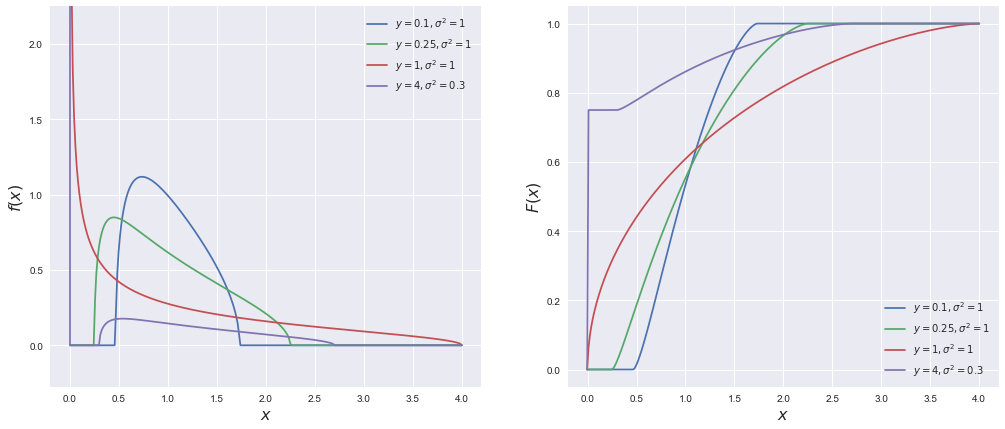
\includegraphics[scale=0.4]{MP}
			\caption{Marchenko-Pastur law}
			\smallskip
			\small
			The left panel shows graphs of the density function $f(x)$ for different parameters $y$ and $\sigma^2$. On the right there are graphs of corresponding cumulative distribution functions $F(x)$. Notice that as $y$ becomes larger the eigenvalues of $\Sigma_p$ spread out instead of concentrating near $\sigma^2$ and the length of the density's support increases.
		\end{center}
	\end{figure}
	
	\begin{rmrk} \
		\begin{enumerate}
			\item We have for $\Sigma_p = \sigma^2 \mathbb{I}_{p \times p}$ the density of limiting spectral distribution
			\[ dH(x) = \delta_{\sigma^2}(x). \]
			Define $m_{\mathcal{MP}}(z)$ as the Stieltjes transform of the Marchenko-Pastur distribution. Then it satisfies the self-consistent equation
			\[
			\begin{aligned}
			m_{\mathcal{MP}}(z) & = \int_{\tau \in \MR} \frac{1}{ \tau( 1-y-zm_{\mathcal{MP}}(z))-z} \delta_{\sigma^2}(x) dx \\
			& =  \frac{1}{ \sigma^2( 1-y-zm_{\mathcal{MP}}(z))-z}.
			\end{aligned}
			\]
			\item Note again that for $y \rightarrow 0$ the density in Proposition \ref{one-dim MP} is
			\[f(x) = \delta_{\sigma^2}(x), \]
			which coincides with the density in Example \ref{ESD finite p} for finite value of $p$ and with density $dH(x)$, because in this case $\Sigma_p^{RCV}$ converges to $\Sigma_p$.
			\item One can show that
			\[ m_{\mathcal{MP}}(z) = \frac{\sigma^2(1-y)-z+ i \sqrt{(b-z)(z-a)}}{2yz}. \]
			Therefore, one can find $m_{\mathcal{MP}}(z)$ through \eqref{Stieltjes transform eig} and derive $\sigma^2$ from it easily.
		\end{enumerate}
		\begin{proof}
			See, e.g., Lemma 2.18 in Ben Adlam
		\end{proof}
	\end{rmrk}
	
	\section*{Non-constant volatility case}
	\begin{rmrk}
		In practice, the covolatility process is typically not constant. Furthermore, stock volatility might not only vary in time, but also be random and depend on the price process itself. In general, for any time-varying covolatility process $\Theta(t)$, we associate it with a constant covolatility process given by the square root of the ICV matrix
		\[ \Theta^0(t) = \sqrt{\int_0^1\Theta(s) \cdot \Theta^T(s) ds} \quad \forall t \in [0, 1]. \]
		Let $\mathbf{X}^0(t)$ be such that
		\[ d\mathbf{X}^0(t) = \Theta^0(t) d\mathbf{W}(t). \]
		Note that $\mathbf{X}(t)$ and $\mathbf{X}^0(t)$ share the same ICV matrix at time 1:
		\[ \Sigma_p^0 :=  \int_0^1 \Theta^0(t) \cdot {\Theta^0}^T(t) dt = \int_0^1 dt \int_0^1\Big( \Theta(s) \cdot {\Theta}^T(s)\Big) ds = \Sigma_p.  \]
		Based on $\mathbf{X}^0(t)$, we have an associated RCV matrix
		\[ \Sigma_p^{RCV^0} = \sum_{\ell=1}^{n} \Delta \mathbf{X}_\ell^0 (\Delta \mathbf{X}_\ell^0)^T. \]
		Since $\Sigma_p^{RCV}$ and $\Sigma_p^{RCV^0}$ are based on the same estimation method and share the same targeting ICV matrix, it is desirable that their ESDs have similar properties. In particular, based on the results in LDRMT and the discussion about constant covolatility case, we have the following property for $\Sigma_p^{RCV^0}$: if the ESD $F^{\Sigma_p}$ converges, then so does $F^{\Sigma_p^{RCV^0}}$. Furthermore, their limits are related to each other via the Marchenko-Pastur equation \eqref{MP eq}. The question is: does this property hold for ESD of $\Sigma_p^{RCV}$? Later we will see that even in the most ideal case, when the covolatility process has the form $\Theta(t) =\gamma(t) \mathbb{I}_{p \times p}$ for some deterministic scalar function $\gamma(t)$, such convergence results may \textit{not} hold for $\Sigma_p^{RCV}$. Moreover, the limit of $F^{\Sigma_p^{RCV}}$ (when it exists) changes according to how the covolatility process evolves over time.
	\end{rmrk}
	
	\begin{defn}
		Let $A$, $B$ be two symmetric $p \times p$ matrices. Then we write
		\[ A \succeq B\]
		to denote that $A-B$ is a positive semidefinite matrix. Similarly, we say that $A \preceq B$ if $A-B$ is negative semidefinite. The partial ordering defined by $\succeq$ is called L\"owner ordering.
	\end{defn}
	
	\begin{lmm}[Weyl's Monotonicity Theorem]
		Suppose $A$ and $B$ are symmetric, $p \times p$ matrices. Let $\lambda_i(A)$ be the $i$-th largest eigenvalue of $A$. If $A \preceq B$, then $\lambda_i(A) \leq \lambda_i(B)$ for all $i$, or, equivalently
		\[ F^B(x) \leq F^A(x) \quad \forall x \geq 0. \]
    \end{lmm}
    \begin{proof}
    	Corollary 4.3.3 in Horn and Johnson (1990).
    \end{proof}
		
	\begin{prps} \label{counter RCV}
		Suppose that for any $p$, $\mathbf{X}(t)$ is a $p$-dimensional process satisfying
		\begin{equation}
		d \mathbf{X}(t) = \gamma(t) d\mathbf{W}(t), \quad t \in [0, 1],
		\end{equation}
		where $\gamma(t) > 0$ is a nonrandom (scalar) c$\grave{\text{a}}$dl$\grave{\text{a}}$g process. Let $\sigma^2 = \int_0^1 \gamma^2(t) dt$ and so that the ICV matrix $\Sigma_p = \sigma^2 \mathbb{I}_{p \times p}$. Assume further that the observation times $\tau_{\ell}$ are equally spaced, that is, $\tau_{\ell} = \ell / n$, and that the RCV matrix $\Sigma_p^{RCV}$ is defined by \eqref{RCV}. Then so long as $\gamma(t)$ is not constant on $[0, 1)$, for any $\varepsilon > 0$, there exists $y_c = y_c(\gamma, \varepsilon) > 0$ such that if $\lim p/n = y \geq y_c$,
		\begin{equation}
			\limsup F^{\Sigma_p^{RCV}}(b(y)+\sigma^2\varepsilon) < 1 \quad \text{a.s.}
		\end{equation}
		In particular, $F^{\Sigma_p^{RCV}}$ doesn't converge to the Marchenko-Pastur law $\mathcal{MP}(y, \sigma^2)$.
    \end{prps}
    
    \begin{proof}
    	By assumption if $\gamma(t)$ is non-contant, there exists $\delta > 0$ and an interval $[c, d] \subseteq [0, 1] $ such that
    	\[ \gamma(t) \geq \sigma(1+\delta) \quad \forall t \in [c, d]. \]
    	Therefore, if $\big[ \frac{\ell - 1}{n}, \frac{\ell}{n} \big] \subseteq [c, d] $ for some $1 \leq \ell \leq n$, then
    	\[ \Delta \mathbf{X}_\ell (\Delta \mathbf{X}_\ell )^T \stackrel{d}{=} \int_{(\ell-1)/n}^{\ell/n} \gamma^2(t) dt \cdot \mathbf{Z}_\ell(\mathbf{Z}_\ell)^T \succeq \frac{(1+\delta)^2}{n} \sigma^2 \mathbf{Z}_\ell(\mathbf{Z}_\ell)^T,  \]
    	where $\mathbf{Z}_\ell = (Z_{1\ell}, \dots , Z_{p\ell})^T$ consists of independent standard normals. Hence, if we let $ J_n = \big\{ \ell: \big[ \frac{\ell - 1}{n}, \frac{\ell}{n} \big] \subseteq [c, d] \big\} $ and
    	\[ \Gamma_p = \sum_{\ell \in J_n} \Delta \mathbf{X}_\ell (\Delta \mathbf{X}_\ell )^T, \quad \Lambda_p = \frac{\sigma^2}{n(d-c)} \sum_{\ell \in J_n} \mathbf{Z}_\ell (\mathbf{Z}_\ell )^T,  \]
    	then for any $x \geq 0$, by Weyl's Monotonicity Theorem,
    	\[
    	F^{\Sigma_p^{RCV}}(x) \leq F^{\Gamma_p}(x) \leq F^{\Lambda_p}\bigg(\frac{x}{(1+\delta)^2(d-c)}\bigg).
    	\]
	    Now note that $\# J_n \sim (d-c)n$, hence if $p/n \rightarrow y$, by Proposition \ref{MP law}, $F^{\Lambda_p}$ will converge a.s. to the Marchenko-Pastur law with ratio index $y'=\frac{y}{d-c}$ and scale index $\sigma^2$.
	    By the formula of $b(\cdot)$ in Marchenko-Pastur density
	    \[
	    \begin{aligned}
	    (1+\delta)^2(d-c)b(y') &=(1+\delta)\sigma^2 \cdot (1+\delta)(d-c)(1+2\sqrt{y'}+y') \\
	    & =(1+\delta)\sigma^2 \cdot (1+\delta)(d-c + 2\sqrt{(d-c)y} + y) \\
	    & := (1+\delta)\sigma^2 \cdot  g(y).
	    \end{aligned}
	    \]
	    Note that the $g(y)$ has a linear growth in $y$ with coefficient $1+\delta$. Hence, for any $\varepsilon > 0$, there exists $y_c > 0$, such that for all $y \geq y_c$
	    \[ g(y) \geq (1+\sqrt{y})^2+\varepsilon,  \]
	    that is,
	    \[ (1+\delta)^2(d-c)b(y') \geq (1+\delta) \sigma^2 \cdot ((1+\sqrt{y})^2+\varepsilon) = (1+\delta)(b(y)+\sigma^2\varepsilon)  \]
	    or, equivalently,
	    \[ \frac{b(y) + \sigma^2\varepsilon}{(1+\delta)^2(d-c)} \leq \frac{b(y')}{1+\delta}. \]
	    Therefore, when the above inequality holds,
	    \[\limsup F^{\Sigma_p^{RCV}}(b(y) + \sigma^2\varepsilon) \leq \limsup F^{\Lambda_p}\bigg(\frac{b(y')}{1+\delta}\bigg) < 1. \]
    \end{proof}
    
    \begin{rmrk}
    	In the proof of Proposition \ref{counter RCV} we saw that more volatility process vary in time, the bigger value of $\delta$ can be found, and hence more the maximum value of domain of $F^{\Sigma_p^{RCV}}$ goes away from $b(y)$. Therefore ESD of $\Sigma_p^{RCV}$ cannot be considered as consistent estimator anymore. In the next part we will study different estimator, which is based on the whole behavior of volatility process.
    \end{rmrk}
    
    \pagebreak
    \part{Limit theorems for non-constant covolatility processes}
    
    \section*{Limiting distribution for realized covariance}
    \begin{rmrk}
    	In this part we will state two major theorems. The first one is a generalization of Proposition \ref{MP law} for limiting spectral distribution of RCV matrix in the case of non-constant covolatility. The second theorem claims the convergence of ESD of alternative estimator to Marchenko-Pastur law. Both theorems require some additional assumptions.
    \end{rmrk}
    
    
    \begin{defn}
    	Suppose that for all $p$ $\mathbf{X}(t) = \mathbf{X}^{(p)}(t)$ is a $p$-dimensional process satisfying \eqref{X diffeq}, and $\Theta(t)$ is c$\grave{\text{a}}$dl$\grave{\text{a}}$g. We say that $\mathbf{X}(t)$ belongs to \define{class $\mathcal{C}$} if, almost surely, there exist $\gamma(t): [0, 1] \mapsto \MR$ and $\Lambda$ a $p \times p$ matrix satisfying $\tr(\Lambda \Lambda^T) = p$ such that 
    	\begin{equation} \label{class C cov}
    	\Theta(t) = \gamma(t) \Lambda.
    	\end{equation}
    	Observe that if \eqref{class C cov} holds, then the ICV matrix $\Sigma_p = \int_{0}^{1} \gamma^2(t) dt \cdot \Lambda \Lambda^T$. The special case when $\Lambda = \mathbb{I}_{p \times p}$ will be studied in simulations.
    \end{defn}
    
    \begin{exmp} \label{exmp C}
    	Suppose that $X_j(t)$ satisfy
    	\[ dX_j(t) = \mu_j(t) dt + \sigma_j(t) dW_j(t), \quad j = 1, \dots, p, \]
    	where $\mu_j(t), \sigma_j(t) : [0, 1] \rightarrow \MR$ are the drift and volatility processes for stock $j$, and $W_j(t)$'s are  (one-dimensional) standard Brownian motions. If the following conditions hold:
    	\begin{itemize}
    		\item the correlation matrix process of $(W_j(t))$
    		\[ R(t):= \bigg(\frac{ [W_j, W_k](t) \ }{t}\bigg)_{1 \leq j,k \leq p} =:(r_{jk})_{1 \leq j,k \leq p} \]
    		is constant in $t \in [0, 1]$.
    		\item $r^{(jk)} \neq 0$ for all $1 \leq j,k \leq p$; and
    		\item the correlation matrix process of $X_j(t)$
    		\[ \Bigg( \frac{\int_{0}^{t} \sigma_j(s) \sigma_k(s)  d[W_j, W_k](s) }{\sqrt{\int_{0}^{t} \sigma_j^2(s) ds \cdot \int_{0}^{t} \sigma_k^2(s) ds}} \Bigg)_{1 \leq j,k \leq p}  =:(\rho_{jk})_{1 \leq j,k \leq p}  \]
    		is constant in $t \in [0, 1]$;
    	\end{itemize}
    	then $\mathbf{X}(t)$ belongs to class $\mathcal{C}$.
    	
    	\begin{proof}
    		For any $t \in [0, 1]$: 
    		\[ \rho_{jk} = \frac{r_{jk} \int_{0}^{t} \sigma_j(s) \sigma_k(s) ds }{\sqrt{\int_{0}^{t} \sigma_j^2(s) ds \cdot \int_{0}^{t} \sigma_k^2(s) ds}}, \]
    		therefore
    		\[ \frac{\rho_{jk}}{r_{jk}} = \frac{\int_{0}^{t} \sigma_j(s) \sigma_k(s) ds/t }{\sqrt{\int_{0}^{t} \sigma_j^2(s) ds/t \cdot \int_{0}^{t} \sigma_k^2(s) ds/t}}. \]
    		Letting $t \downarrow 0$, using l'H$\hat{\text{o}}$pital's rule and noting that $\sigma_j(t)$ are c$\grave{\text{a}}$dl$\grave{\text{a}}$g, we observe that
    		\[ \frac{\rho_{jk}}{r_{jk}} = \frac{\sigma_j(0) \sigma_k(0)}{ \sqrt{\sigma_j^2(0) \cdot \sigma_k^2(0) }} = \pm 1. \]
    		Hence, for all $t \in [0, 1]$:
    		\[ \bigg| \int_{0}^{t}\sigma_j(s) \sigma_k(s) ds \bigg| = \sqrt{\int_{0}^{t} \sigma_j^2(s) ds \cdot \int_{0}^{t} \sigma_k^2(s) ds} . \]
    		By Cauchy-Schwartz inequality, this holds only if $\sigma_j(s)$ and $\sigma_k(s)$ are proportional to each other. Therefore, almost surely, there exists a scalar process $\gamma(t) : [0, 1] \rightarrow \MR$ and a $p$-dimensional vector $(\sigma_1, \dots, \sigma_p)^T$, such that
    		\[ (\sigma_1(t), \dots, \sigma_p(t))^T = \gamma(t) \cdot (\sigma_1, \dots, \sigma_p)^T. \]
    		Now we show that $\mathbf{X}(t)$ belongs to class $\mathcal{C}$. In fact one can always find a $p$-dimensional standard Brownian motion $\widetilde{\mathbf{W}}(t)$, such that 
    		\[ \mathbf{W}(t) = R^{1/2}\widetilde{\mathbf{W}}(t), \]
    		where $\mathbf{W} = (W_1(t), \dots, W_p(t))^T$ and $R$ is a correlation matrix of $\mathbf{W}(t)$, which is constant for all $t \in [0, 1]$ by assumption. Hence, writing $\mu(t) = (\mu_1(t), \dots, \mu_p(t))^T$, we have
    		\[ 
    		\begin{aligned}
    		d\mathbf{X}(t) & = \mu(t) dt + \diag(\sigma_1(t), \dots, \sigma_p(t)) d\mathbf{W}(t) \\
    		&  = \mu(t) dt +\gamma(t) \cdot \diag(\sigma_1, \dots, \sigma_p) R^{1/2} d\widetilde{\mathbf{W}}(t).
    		\end{aligned} \]
    	\end{proof}
    \end{exmp}
    
    \begin{rmrk} \
    	\begin{enumerate}
    		\item In particular, if all Brownian motions in Example \ref{exmp C} are independent of each other, then $R(t)$ is an identity matrix $\mathbb{I}_{p \times p}$. Then correlation matrix process of $X_j(t)$ is a diagonal matrix and we need only to require $\rho_{jj}$ to be constant in $t$. 
    		\item The process in Example \ref{exmp X3} doesn't belong to the class $\mathcal{C}$, because its correlation structure varies in time.
    		\item Observe that if a diffusion process $\mathbf{X}(t)$ belongs to class $\mathcal{C}$, the drift process $\boldsymbol{\mu}(t) = 0$, and $\tau_\ell$'s and $\gamma(t)$ are independent of $\mathbf{W}(t)$, then
    		\[ \Delta \mathbf{X}_\ell = \int_{\tau_{\ell-1}}^{\tau_\ell} \gamma(t) \Lambda d\mathbf{W}(t) \stackrel{d}{=} \sqrt{\int_{\tau_{\ell-1}}^{\tau_\ell} \gamma^2(t)dt} \cdot \overline{\Sigma}^{1/2} \cdot \mathbf{Z}_\ell, \]
    		where $ \overline{\Sigma}^{1/2}$ is the nonnegative square root matrix of
    		\[\overline{\Sigma} := \Lambda \Lambda^T \]
    		and $\mathbf{Z}_\ell = (Z_{1\ell}, \dots, Z_{p\ell})^T$ consists of independent standard normals. Therefore, the RCV matrix
    		\[ \Sigma_p^{RCV} = \sum_{\ell=1}^{n} \Delta \mathbf{X}_\ell(\Delta \mathbf{X}_\ell)^T \stackrel{d}{=} \sum_{\ell=1}^{n} w_\ell^n \cdot \overline{\Sigma}^{1/2}\mathbf{Z}_\ell (\mathbf{Z}_\ell)^T \overline{\Sigma}^{1/2} \]
    		with 
    		\[w_\ell^n =\int_{\tau_{\ell-1}}^{\tau_\ell} \gamma^2(t)dt.\]
    		This is similar to the $S_p$ in Proposition \ref{MP law}, except that here the weights $w_\ell^n$ may vary in $\ell$, while in Proposition \ref{MP law} the weights are constantly $1/n$.
    	\end{enumerate}
    \end{rmrk}
    
    \begin{rmrk}
    	In order to avoid confusion, we should specify the designations. For any vector $A = (A_1, \dots, A_n)^T$, $\|A\|_2$ denotes its $L^2$-norm, that is
    	\[ \|A\|_2 = \sqrt{\sum_{\ell=1}^n A_\ell^2 }. \]
    	Note that
    	\[ \|A\|_2^2 = A^T A. \]
    	Let $\mathbf{A}$ be $m \times n$ matrix and $\mathbf{A}^* = \overline{\mathbf{A}^T}$ its conjugate transpose. Let also $\lambda_{\max}(\cdot)$ be the operator, taking the largest eigenvalue. Then
    	\[ \|\mathbf{A} \| = \sqrt{\lambda_{\max} (\mathbf{A}^* \mathbf{A}) } \]
    	denote a spectral norm of $\mathbf{A}$. The value $\lambda_{\max} (\mathbf{A}^* \mathbf{A})$ is also called singular value of the matrix $\mathbf{A}$.
    \end{rmrk}
    
    \begin{thm} \label{Thm 1}
    	Assume that all the conditions in Proposition \ref{MP law} are satisfied. Furthermore,
    	\begin{enumerate}
    		\item $Z_{j\ell}^{(p)}$ have finite moments of all orders;
    		\item $H$ has a finite second moment;
    		\item the weights $w_\ell^n$, $1 \leq \ell \leq n$, $n = 1, 2, \dots$, are all positive, and there exists $\kappa < \infty$ such that the rescaled weights $(nw_\ell^n)$ satisfy
    		\[ \max_n \max_{\ell = 1, \dots, n} (nw_\ell^n) \leq \kappa; \]
    		moreover, almost surely, there exists a c$\grave{\text{a}}$dl$\grave{\text{a}}$g function $w(s): [0, 1] \rightarrow \MR_{+}$, such that
    		\[ \lim_n \sum_{1 \leq \ell \leq n} \int_{(\ell-1)/n}^{\ell/n} |n w_\ell^n - w(s)|ds = 0; \]
    		\item there exists a sequence $\eta_p = o(p)$ and a sequence of index sets $\mathcal{I}_p$ satisfying $\mathcal{I}_p \subset \{1, \dots, p\}$ and $\#\mathcal{I}_p \leq \eta_p$ such that for all $n$ and all $\ell$, $w_\ell^n$ may depend on $\mathbf{Z}_\ell^{(p)}$ but only on $\{ Z_{j\ell}^{(p)}: j \in \mathcal{I}_p \}$;
    		\item there exist $C < \infty$ and $\delta < 1/6$ such that for all $p$, $\| \Sigma_p \| \leq Cp^\delta$ a.s.
    	\end{enumerate}
    	Define $S_p = \sum_{\ell=1}^{n} w_\ell^n \cdot \Sigma_p^{1/2} \mathbf{Z}_\ell^{(p)} (\mathbf{Z}_\ell^{(p)})^T\Sigma_p^{1/2} $. Then, almost surely, the ESD of $S_p$ converges in distribution to a probability distribution $F^w$, which is determined by $H$ and $w(s)$ in that its Stiltjes trasform $m_{F^w}(z)$ is given by
    	\[ m_{F^w}(z) = -\frac{1}{z} \int_{\tau \in \MR} \frac{1}{\tau M(z) + 1} dH(\tau), \]
    	where $M(z)$, together with another function $\tilde{m}(z)$, uniquely solve the following equation in $\mathbb{C}_{+} \times \mathbb{C}_{+}$:
    	\[
    	\left \{
    	\begin{array}{l}
    		M(z) = -\frac{1}{z} \int_{\tau \in \MR} \frac{w_s}{1 + y \tilde{m}(z)w_s} ds,  \\
    		\tilde{m}(z) =  -\frac{1}{z} \int_{\tau \in \MR} \frac{\tau}{\tau M(z) + 1} dH(\tau).
    	\end{array}
    	\right.
    	\]
    \end{thm}
    
    \begin{rmrk}
    	If $w_\ell^n = 1/n$, then $w(s)=1$, and Theorem \ref{Thm 1} reduces to Proposition \ref{MP law}. Moreover, if $w(s)$ is not constant, that is, $w(s) \neq \int_{0}^{1} w(t) dt$ on $[0, 1]$, then except in the trivial case when $H$ is a delta measure at $0$, the LSD $F^w \neq F$, where $F$ is the LSD in Proposition \ref{MP law} determined by $H(\cdot / \int_{0}^{1} w(t) dt)$. (ADD MORE EXPLANATION FROM SUPPLEMENTARY ARTICLE)
    \end{rmrk}
    
    \begin{prps}
    	Suppose that for all $p$, $X^{(p)}(t)$ is a $p$-dimensional process in class $\mathcal{C}$ with some drift process $\boldsymbol{\mu}(t) = (\mu_1^{(p)}(t), \dots, \mu_p^{(p)}(t))^T$, covolatility process $\Theta^{(p)}(t) = \gamma^{(p)}(t) \Lambda^{(p)}$ and $p$-dimensional Brownian motion $\mathbf{W}^{(p)}(t) = (W_1^{(p)}(t), \dots, W_t^{(p)}(t) )^T$. Suppose further that:
    	\begin{enumerate}
    		\item there exists $C_0 < \infty$ such that for all $p$ and all $j = 1, \dots, p$, $|\mu_j^{(p)}(t)| \leq C_0$ for all $t \in [0, 1]$ almost surely;
    		\item $\breve{\Sigma}_p = \Lambda^{(p)} ( \Lambda^{(p)})^T $ is (a possibly random) positive semi-definite $p \times p$ matrix such that its ESD $F^{\breve{\Sigma}_p}$ converges almost surely in distribution to a probability distribution $\breve{H}$ on $[0,\infty)$ as $p \rightarrow \infty$; moreover, $\breve{H}$ has a finite second moment;
    		\item there exist $C < \infty$ and $\delta < 1/6$ such that for all $p$, $\|\breve{\Sigma}_p \| \leq Cp^\delta$ almost surely;
    		\item there exits a sequence $\eta_p = o(p)$ and a sequence of index sets $\mathcal{I}_p$ satisfying $\mathcal{I}_p \subset \{1, \dots, p\}$ and $\#\mathcal{I}_p \leq \eta_p$ such that $\gamma^{(p)}(t)$ may depend on $\mathbf{W}^{(p)}(t)$ but only on $\{W_j^{(p)}(t): j \in \mathcal{I}_p\}$; moreover, there exists $C_1 < \infty$ such that for all $p$, $|\gamma^{(p)}(t)| \leq C_1$ for all $t \in [0, 1]$ almost surely; additionally, almost surely, there exists $\gamma(t): [0, 1] \rightarrow \MR$ such that
    		\[ \lim_{p \rightarrow \infty} \int_{0}^{1} |\gamma^{(p)}(t) - \gamma(t) |dt = 0;  \]
    		\item the observation times $\tau_\ell$ are independent of $\mathbf{X}(t)$; moreover, there exists $\kappa < \infty$ such that the observation durations $\Delta \tau_\ell := \tau_\ell - \tau_{\ell-1}$ satisfy
    		\[ \max_{n} \max_{\ell = 1, \dots, n} (n \cdot \Delta \tau_\ell ) \leq \kappa; \]
    		additionally, almost surely, there exists a process $\upsilon(s) : [0, 1] \rightarrow \MR_+$ such that
    		\[ \lim_{n \rightarrow \infty} \tau_{[ns]} = \Upsilon(s) :=\int_{0}^{1} \upsilon(r) dr \quad \forall 0 \leq s \leq 1, \]
    		where for any $x$, $[x]$ stands for its integer part.
     	\end{enumerate}
     	Then, as $p \rightarrow \infty$, $F^{\Sigma_p^{RCV}}$ converges almost surely to a probability distribution $F^w$ as specified in Theorem \ref{Thm 1} for
     	\[ w_s = (\gamma(\Upsilon_s))^2 \upsilon(s). \]
    \end{prps}
    
    \begin{rmrk}
    	содержимое...
    \end{rmrk}
    
    \section*{Time-variance adjusted realized covariance}
    		
    \begin{defn}
   		Suppose that a diffusion process $\mathbf{X}(t)$ belongs to class $\mathcal{C}$. We define \define{time-variation adjusted realized covariance (TVARCV) matrix} as follows:
   		\begin{equation} \label{TVARCV}
   		\widehat{\Sigma}_p := \frac{\tr \big( \Sigma_p^{RCV} \big) }{n} \sum_{\ell = 1}^{n} \frac{\Delta \mathbf{X}_\ell (\Delta \mathbf{X}_\ell)^T}{\| \Delta \mathbf{X}_\ell \|_2^2} = \frac{\tr \big( \Sigma_p^{RCV} \big) }{p} \widetilde{\Sigma}_p,
   		\end{equation}
   		where
   		\begin{equation} \label{Sigma_tilde}
   		\widetilde{\Sigma}_p := \frac{p}{n} \sum_{\ell = 1}^{n} \frac{\Delta \mathbf{X}_\ell (\Delta \mathbf{X}_\ell)^T}{\| \Delta \mathbf{X}_\ell \|_2^2}.
   		\end{equation}
    \end{defn}
    
    \begin{rmrk}
    	Let us explain $\widetilde{\Sigma}_p$. Consider the simplest case when $\mu(t) = 0$, $\gamma(t)$ is deterministic, $\Lambda_t = \mathbb{I}_{p \times p}$, and $\tau_{\ell} = \ell / n$, $\ell = 0, 1, \dots, n$. In this case,
    	\[ \Delta \mathbf{X}_\ell = \sqrt{\int_{(\ell - 1)/n}^{\ell / n} \gamma^2(t) dt }\cdot \frac{\mathbf{Z}_\ell}{\sqrt{n}}, \]
    	where $\mathbf{Z}_\ell = (Z_{1\ell}, \dots, Z_{p\ell})^T$ is a vector of i.i.d. standard normal random variables. Hence,
    	\[ \frac{\Delta \mathbf{X}_\ell (\Delta \mathbf{X}_\ell)^T}{\| \Delta \mathbf{X}_\ell \|_2^2} = \frac{\mathbf{Z}_\ell \mathbf{Z}_\ell^T}{\|  \mathbf{Z}_\ell \|_2^2}. \]
    	However, as $p \rightarrow \infty$, $\| \mathbf{Z}_\ell \|_2^2 \sim p$, hence
    	\[ \widetilde{\Sigma}_p \sim \frac{\sum_{\ell = 1}^{n}\mathbf{Z}_\ell \mathbf{Z}_\ell^T}{n}, \]
    	the latter being the usual sample covariance matrix.
    	We will show that, first, $\tr(\Sigma_p^{RCV}) \sim \tr(\Sigma_p)$; and second, if $\mathbf{X}(t)$ belongs to class $\mathcal{C}$ and satisfies certain additional assumptions, then the LSD of $\widetilde{\Sigma}_p$ is related to that of $\breve{\Sigma}_p$ via the Marchenko-Pastur equation, where
    	\[ \breve{\Sigma}_p = \frac{p}{\tr(\Sigma_p)}\Sigma_p = \Lambda \Lambda^T. \]
    	Hence, the LSD of $\widehat{\Sigma}_p$ is also related to that of $\Sigma_p$ via the same Marchenko-Pastur equation.
    	We will now state our assumptions for the major theorem in this paper.
    \end{rmrk}
    
    \begin{asmp} \label{asmp2} \
    	\begin{enumerate}
    		\item there exists $C_0 < \infty$ such that for all $p$ and all $j = 1, \dots, p$, $|\mu_j^{(p)}(t)| \leq C_0$ for all $t \in [0, 1]$ a.s.;
    		\item there exist constants $C_1 < \infty$, $0 \leq \delta_1 < 1/2$, a sequence $\eta_p < C_1 p^{\delta_1}$ and a sequence of index sets $\mathcal{I}_p$ satisfying $\mathcal{I}_p \subset \{ 1, \dots p \}$ and $\# \mathcal{I}_p \leq \eta_p$ such that $\gamma^{(p)}(t)$ may depend on $\mathbf{W}^{(p)}(t)$ but only on $\{ W_j^{(p)}(t) : j \in \mathcal{I}_p \}$; moreover, there exists $C_2 < \infty$ such that for all $p$, $|\gamma^{(p)}(t)| \in (1/C_2, C_2)$ for all $t \in [0, 1]$ a.s.;
    		\item there exists $C_3 < \infty$ such that for all $p$ and for all $j$, the individual volatilities \[ \sigma_j(t) = \gamma^{(p)}(t)\sqrt{\sum_{k=1}^{p} (\Lambda_{jk}^{(p)})^2} \in (1/C_3, C_3)\] for all $t \in [0, 1]$ a.s.;
    		\item \[ \lim_{p \rightarrow \infty} \frac{\tr(\Sigma_p)}{p} = \lim_{p \rightarrow \infty} \int_{0}^{1} (\gamma^{(p)}(t))^2 dt := \theta > 0 \quad \text{a.s.}; \]
    		\item almost surely, as $p \rightarrow \infty$, the ESD $F^{\Sigma_p}$ converges to a probability distribution $H$ on $[0, \infty)$;
    		\item there exist $C_5 < \infty$ and $0 \leq \delta_2 < 1/2$ such that for all $p$, $\| \Sigma_p \| \leq C_5 p^{\delta_2}$ a.s.;
    		\item the $\delta_1$ in (ii) and $\delta_2$ in (vi) satisfy that $\delta_1 + \delta_2 < 1/2$;
    		\item $p/n \rightarrow y \in (0, \infty) $ as $p \rightarrow \infty$; and
    		\item there exists $C_4 < \infty$ such that for all $n$,
    		\[ \max_{1 \leq \ell \leq n} n \cdot (\tau_{\ell} - \tau_{\ell - 1}) \leq C_4 \quad \text{a.s.}  \]
    		moreover, $\tau_{\ell}$'s are independent of $\mathbf{X}(t)$.
    	\end{enumerate}
    \end{asmp}
    
    \begin{rmrk}
    	Before stating and proving theorem for TVARCV we provide some useful lemmas.
    \end{rmrk}
    
    \begin{lmm}[Burkholder-Davis-Gundy inequality] \label{BDG}
    	For any real number $p \geq 1$ there exist positive constants $c_p$ and $C_p$ such that, for all local martingales $X(t)$ with $X(0) = 0$, its maximum processes $M(t) = \sup_{t \leq s} |X(s)|$ and stopping times $\tau$, the following inequalities hold
    	\[ c_p \ME[[X]^{p/2}(\tau)] \leq \ME[M^p(\tau)] \leq C_p \ME[[X]^{p/2}(\tau)]. \]
    \end{lmm}
    \begin{proof}
    	LOOK IN THE BOOKS
    \end{proof}
    
    \begin{defn}
    	Let $F$ and $G$ be two cumulative distribution functions. Then the L$\acute{\text{e}}$vy distance between them is
    	\[ L(F, G) := \inf \{ \varepsilon > 0 : F(x-\varepsilon) -\varepsilon \leq G(x) \leq F(x+\varepsilon) + \varepsilon \quad \forall x\in\MR   \} \]
    \end{defn}
    
    \begin{lmm} \label{lmm1}
    	Suppose that for each $p$, $\mathbf{v}_\ell^{(p)} = (v_{1\ell}^{(p)}, \dots, v_{p\ell}^{(p)})^T$ and $\mathbf{w}_\ell^{(p)} = (w_{1\ell}^{(p)}, \dots, w_{p\ell}^{(p)})^T$, $\ell = 1, \dots, n$, are all $p$-dimensional vectors. Define
    	\[	\widetilde{S}_n = \sum_{\ell = 1}^{n} (\mathbf{v}_\ell^{(p)} + \mathbf{w}_\ell^{(p)}) \cdot (\mathbf{v}_\ell^{(p)} + \mathbf{w}_\ell^{(p)})^T\]
    	and
    	\[S_n = \sum_{\ell = 1}^{n} \mathbf{w}_\ell^{(p)} (\mathbf{w}_\ell^{(p)})^T. \]
    	If the following conditions are satisfied:
    	\begin{enumerate}
    		\item $\lim_{p \rightarrow \infty} p/n = y > 0$;
    		\item there exists a sequence $\varepsilon_p = o(1/\sqrt{p})$ such that for all $p$ and all $\ell$, all the entries of $\mathbf{v}_\ell^{(p)}$ are bounded by $\varepsilon_p$ in absolute value;
    		\item $ \limsup_{p \rightarrow \infty} {\tr(S_n)}/{p} < \infty$ almost surely.
    	\end{enumerate}
    	Then $L(F^{\widetilde{S}_n}, F^{S_n}) \rightarrow 0$ almost surely.
    \end{lmm}
    \begin{proof}
    	For notational ease we shall omit the superscript $p$ and write $\mathbf{v}_\ell = \mathbf{v}_\ell^{(p)}$, $\mathbf{w}_\ell = \mathbf{w}_\ell^{(p)}$, $v_{j\ell} = v_{j\ell}^{(p)}$, etc. For each $p$ set 
    	\[ A = A_p = (\mathbf{v}_1 + \mathbf{w}_1, \dots, \mathbf{v}_n + \mathbf{w}_1) \]
    	and
    	\[ B = B_p = (\mathbf{w}_1, \dots,  \mathbf{w}_n). \]
    	Then
    	\[ \widetilde{S}_n = A A^T \quad \text{and} \quad S_n = BB^T. \]
    	By Lemma 2.7 of Bai (1999)
    	\[L^4(F^{\widetilde{S}_n}, F^{S_n}) \leq \frac{2}{p^2} \tr((A-B)(A-B)^T) \cdot \tr(\widetilde{S}_n + S_n). \]
    	By condition (ii),
    	\[ \tr((A-B)(A-B)^T)  = \sum_{\ell=1}^{n} \sum_{j=1}^{p} v_{j\ell}^2 \leq np \cdot \varepsilon_p^2. \]
    	Moreover,
    	\[
    	\begin{aligned}
    	\tr(\widetilde{S}_n) &= \sum_{\ell=1}^{n} \sum_{j=1}^{p} (v_{j\ell} + w_{j\ell})^2 \\
    	& \leq 2 \sum_{\ell=1}^{n} \sum_{j=1}^{p} v_{j\ell}^2 + 2\sum_{\ell=1}^{n} \sum_{j=1}^{p} w_{j\ell}^2 \\
    	& \leq 2np \cdot \varepsilon_p^2 + 2 \tr(S_n).
    	\end{aligned}
    	 \]
    	 Therefore,
    	 \[L^4(F^{\widetilde{S}_n}, F^{S_n}) \leq 4n^2\varepsilon_p^4 + 6n\varepsilon_p^2 \frac{\tr(S_n)}{p}. \]
    	 The conclusion follows since $\varepsilon_p = o(1/\sqrt{p})$ and hence $o(1/\sqrt{n})$.
    \end{proof}
    
    \begin{lmm} \label{trace conv}
    	Under Assumptions \ref{asmp2}(iv), namely, suppose that
    	\[ \lim_{p \rightarrow \infty} \frac{\tr(\Sigma_p)}{p} = \theta \quad \text{a.s.}, \]
    	then
    	\[ \lim_{p \rightarrow \infty} \frac{\tr(\Sigma_p^{RCV})}{p} = \theta \quad \text{a.s.} \]
    \end{lmm}
    \begin{proof}
    	The full proof can be found in supplementary article OF THE PAPER .... We will provide here the main idea: it suffices to show that
    	\[ \frac{\tr(\Sigma_p^{RCV})-\tr(\Sigma_p)}{p} \xrightarrow[p \rightarrow \infty]{} 0 \quad \text{a.s.} \]
    	Let us first consider one-dimensional process
    	\[ dX(t) = \mu(t)dt + \sigma(t)dW(t). \]
    	Under slight assumptions it can be shown that there exist constants $c$, $C_1$ and $C_2$, such that for all $0 \leq x \leq c \sqrt{n}$
    	\[\MP\Big(\sqrt{n} \Big| [X, X](1) - \int_{0}^{1} \sigma^2(t)dt \Big| \geq x \Big) \leq C_1 \exp \{ -C_2 x^2 \}. \]
    	Therefore, generalizing it for $p$-dimensional processes, we have for every $1 \leq j \leq p$
    	\[ \MP(\sqrt{n} |(\Sigma_p^{RCV})_{jj} - (\Sigma_p)_{jj} | > x) \leq C_1 \exp \{ -C_2 x^2 \}. \]
    	Hence, for any $0 < \varepsilon < c$ and for all $p$,
    	\[ 
    	\begin{aligned}
    	\MP \Bigg(  \Bigg| \frac{\tr(\Sigma_p^{RCV})-\tr(\Sigma_p)}{p}  \Bigg| \geq \varepsilon \Bigg) & \leq \sum_{j=1}^{p} \MP(\sqrt{n} |(\Sigma_p^{RCV})_{jj} - (\Sigma_p)_{jj} | \geq \varepsilon) \\
    	& \leq p \cdot C_1 \exp \{ -C_2 \varepsilon^2 \cdot n  \}.
    	\end{aligned}
    	\]
    	The almost sure convergence then follows from the Borel-Cantelli lemma\footnote{
    		Let $X_1, X_2, \dots$ be a sequence of random variables in some probability space and $\varepsilon > 0$ be arbitrary.
    		Then
    		\[ \sum_{n=1}^{\infty} \MP(|X_n| \geq \varepsilon) < \infty \Longrightarrow X_n \xrightarrow{a.s.} 0.  \]
    	}.
    \end{proof}
    
    \begin{crlr} \label{crlr trace conv}
    	The main results of the Lemma \ref{trace conv} are the convergence of $\breve{\Sigma}_p$ 
    	\[ \lim_{p \rightarrow \infty} \breve{\Sigma}_p \rightarrow \frac{1}{\theta} \Sigma_p \]
    	and of TVARCV estimator
    	\[ \lim_{p \rightarrow \infty} \widehat{\Sigma}_p \rightarrow \theta \widetilde{\Sigma}_p. \]
    \end{crlr}
    
    \begin{rmrk} \label{Thm 2 expl}
    	Using Lemma \ref{trace conv} we state that ESD of $\breve{\Sigma}_p$ converges almost surely:
    	\[\lim_{p,n \rightarrow \infty} F^{\breve{\Sigma}_p} \rightarrow \breve{H} \quad \text{a.s.},\] 
    	where $\breve{H}$ is defined by
    	\[\breve{H}(x) = H(\theta x) \quad \forall x \geq 0. \]
    	It is obvious, since
    	\[ F^{\breve{\Sigma}_p} = F^{\Sigma_p}(\tr(\Sigma_p)/p \cdot x) \quad \forall x \geq 0. \]
    	Now it is left to prove the following:
    	\[\lim_{p,n \rightarrow \infty}   F^{\widetilde{\Sigma}_p} \rightarrow \widetilde{F} \quad \text{a.s.}, \]
    	where the LSD $\widetilde{F}$ of $\widetilde{\Sigma}_p$ is determined by $\breve{H}$ in that its Stieltjes transform $m_{\widetilde{F}}(z)$ satisfies the equation
    	\[ m_{\widetilde{F}}(z) = \int_{\tau \in \MR} \frac{1}{ \tau(1- y(1 + zm_{\widetilde{F}}(z))) - z } d\breve{H}(\tau). \]
    	Then the convergence of $\widehat{\Sigma}_p$ will follow from the Corollary \ref{crlr trace conv}.
    \end{rmrk}
    
    \begin{thm} \label{Thm 2}
    	Suppose that for all $p$, $\mathbf{X}(t) = \mathbf{X}^{(p)}(t)$ is a $p$-dimensional process in class $\mathcal{C}$ for some drift process $\boldsymbol{\mu}^{(p)}(t) = (\mu_1^{(p)}(t), \dots , \mu_p^{(p)}(t))^T$, covolatility process $\Theta^{(p)}(t) = \gamma^{(p)}(t) \Lambda^{(p)}$ and a $p$-dimensional Brownian motion $\mathbf{W}_t^{(p)}$, which satisfy Assumptions \ref{asmp2} (i)-(vii) above. Suppose also that $p$ and $n$ satisfy Assumptions \ref{asmp2} (viii), and the observation times satisfy Assumptions \ref{asmp2} (ix). Let $\hat{\Sigma}_p$ be as in \eqref{TVARCV}. Then, as $p \rightarrow \infty$, $F^{\hat{\Sigma}_p}$ converges a.s. to a probability distribution $F$, which is determined by $H$ through Stieltjes transforms via the same Marchenko-Pastur equation as in Proposition \ref{MP law}.
    \end{thm}
    \begin{proof}
    	We only need to show the convergence of $F^{\widetilde{\Sigma}_p}$. For notational ease, we shall omit the superscript $p$ in the arguments below: thus we write $\boldsymbol{\mu}(t)$ instead of $\boldsymbol{\mu}^{(p)}(t)$, $\gamma(t)$ instead of $\gamma^{(p)}(t)$, $\Lambda$ instead of $\Lambda^{(p)}$, etc. First, note that
    	\[ \Delta \mathbf{X}_\ell = \int_{\tau_{\ell-1}}^{\tau_\ell} \boldsymbol{\mu}(t) dt + \Lambda \cdot \int_{\tau_{\ell-1}}^{\tau_\ell} \gamma(t) d\mathbf{W}(t) := \sqrt{\int_{\tau_{\ell-1}}^{\tau_\ell} \gamma^2(t) dt}\cdot (\mathbf{v}_\ell + \Lambda \cdot \mathbf{Z}_\ell), \]
    	where
    	\[ \mathbf{v}_\ell = (v_{1\ell}, \dots, v_{p\ell})^T = \frac{\int_{\tau_{\ell-1}}^{\tau_\ell} \boldsymbol{\mu}(t) dt}{\sqrt{\int_{\tau_{\ell-1}}^{\tau_\ell} \gamma^2(t) dt}} \]
    	and
    	\[ \mathbf{Z}_\ell = (Z_{1\ell}, \dots, Z_{p\ell})^T = \frac{\int_{\tau_{\ell-1}}^{\tau_\ell} \gamma(t) d\mathbf{W}(t)}{\sqrt{\int_{\tau_{\ell-1}}^{\tau_\ell} \gamma^2(t) dt}} \]
    	By performing an orthogonal transformation if necessary, w.l.o.g., we may assume that the index set $\mathcal{I}_p \subset \{ 1, \dots, \eta_p \} $. Then by Assumptions \ref{asmp2} (ii) and (ix), for $j > \eta_p$, $Z_{j\ell}$ are i.i.d. $\sim \mathcal{N}(0, 1)$. Write
    	\[ \mathbf{U}_\ell = (Z_{1\ell}, \dots Z_{\eta_p\ell})^T \]
    	and 
    	\[ \mathbf{D}_\ell = (Z_{\eta_{p}+1\ell}, \dots Z_{p\ell})^T.\]
    	With the above notation, $\widetilde{\Sigma}_p$ can be rewritten as
    	\begin{equation}
    	\widetilde{\Sigma}_p = y_n \sum_{\ell=1}^{n} \frac{\Delta \mathbf{X}_\ell (\Delta \mathbf{X}_\ell)^T}{\|\Delta \mathbf{X}_\ell\|_2^2} = y_n \sum_{\ell=1}^{n} \frac{(\mathbf{v}_\ell + \Lambda \mathbf{Z}_\ell) (\mathbf{v}_\ell + \Lambda \mathbf{Z}_\ell)^T}{\|\mathbf{v}_\ell + \Lambda \mathbf{Z}_\ell\|_2^2}
    	\end{equation}
    	By Assumptions \ref{asmp2} (i), (ii) and (ix), there exists $C > 0$, such that $|v_{j\ell}| \leq C / \sqrt{n}$ for all $j$ and $\ell$, hence $\| \mathbf{v}_\ell\|_2$'s are uniformly bounded. We will show that
    	\begin{equation} \label{334}
    		\max_{\ell = 1, \dots, n} \Bigg|\frac{  \| \Lambda \mathbf{Z}_\ell \|_2^2}{p} - 1\Bigg| = \max_{\ell = 1, \dots, n} \Bigg| \frac{  \mathbf{Z}_\ell^T \breve{\Sigma}_p \mathbf{Z}_\ell}{p} - 1\Bigg| \rightarrow 0 \quad \text{a.s.},
    	\end{equation}
    	which clearly implies that
    	\begin{equation} \label{335}
    		\max_{\ell = 1, \dots, n} \Bigg|\frac{  \| \mathbf{v}_\ell + \Lambda\mathbf{Z}_\ell  \|_2^2}{p} - 1\Bigg| \rightarrow 0 \quad \text{a.s.}
    	\end{equation}
    	To prove \eqref{334} let us write
    	\[ \breve{\Sigma}_p = \begin{pmatrix}
    	A & B \\
    	B^T & C
    	\end{pmatrix}, \]
    	where $A$, $B$ and $C$ are $\eta_p \times \eta_p$, $\eta_p \times (n - \eta_p)$ and $(n-\eta_p) \times (n-\eta_p)$ matrices, respectively. Then
    	\[ \mathbf{Z}_\ell^T \breve{\Sigma}_p \mathbf{Z}_\ell = \mathbf{U}_\ell^T A \mathbf{U}_\ell + 2\mathbf{D}_\ell^T B^T \mathbf{U}_\ell + \mathbf{D}_\ell^T C \mathbf{D}_\ell.  \]    	
    	By a well-known fact about the spectral norm,
    	\[ \|A\| \leq \|\breve{\Sigma}_p \|, \quad \|B\| \leq \|\breve{\Sigma}_p \| \quad \text{and} \quad \|C\| \leq \|\breve{\Sigma}_p \|. \]
    	In particular, by Assumptions \ref{asmp2} (ii), (vi) and (vii),
    	\[ 0 \leq \tr(A) \leq \eta_p \cdot \|\breve{\Sigma}_p \| \leq Cp^{\delta_1 + \delta_2} = o(p), \]
    	hence 
    	\[ \frac{\tr(C)}{p} = \frac{\tr(\breve{\Sigma}_p)-\tr(A)}{p} \rightarrow 1. \]
    	Now using the fact that $\mathbf{D}_\ell$ consists of i.i.d. standard normals and by the same proof as that for (READ THE PROOF AND WRITE IT HERE!!!)
    	we get
    	\[ \max_{\ell = 1, \dots, n} \Bigg| \frac{\mathbf{D}_\ell^T C \mathbf{D}_\ell}{p} - 1 \Bigg| \rightarrow 0 \quad \text{a.s.} \]
    	To complete the proof of \eqref{334}, it then suffices to show that
    	\[ \max_{\ell = 1, \dots, n} \frac{| \mathbf{U}_\ell^T A \mathbf{U}_\ell |}{p} \rightarrow 0 \quad \text{and} \quad \max_{\ell = 1, \dots, n} \frac{| \mathbf{D}_\ell^T B \mathbf{U}_\ell |}{p} \rightarrow 0 \quad \text{a.s.} \]
    	We shall only prove the first convergence, the second one can be proved similarly. We have
    	\begin{equation} \label{337}
    		|\mathbf{U}_\ell A \mathbf{U}_\ell| \leq \|A\| \cdot \|\mathbf{U}_\ell\|_2^2 \leq C_5 p^{\delta_2} \cdot \|\mathbf{U}_\ell\|_2^2
    	\end{equation}
    	Observe that for all $1 \leq i \leq \eta_p$, by Assumptions \ref{asmp2} (ii),
    	\[ | Z_\ell^{(i)} |^2 = \frac{|\int_{\tau_{\ell-1}}^{\tau_\ell} \gamma_t d\mathbf{W}_t|^2}{\int_{\tau_{\ell-1}}^{\tau_\ell} \gamma_t^2 dt} \leq \frac{C_2^2}{\tau_\ell-\tau_{\ell-1} } \cdot \Bigg|\int_{\tau_{\ell-1}}^{\tau_\ell} \gamma_t d\mathbf{W}_t \Bigg|^2. \] 
    	By Lemma \ref{BDG} , we then get that for any $k \in \MN$, there exists $\lambda_k > 0$ such that
    	\begin{equation} \label{338}
    		\ME[ |Z_\ell^{(i)}|^{2k} ] \leq \lambda_k C_2^{4k}.
    	\end{equation}
    	Now we are ready to show that $\max_{\ell = 1, \dots, n} \frac{| \mathbf{U}_\ell^T A \mathbf{U}_\ell |}{p} \rightarrow 0 $. In fact, for any $\varepsilon > 0$, for any $k \in \MN$, by Markov's inequality\footnote{
    		Markov's inequality states that for any non-negative random variable $X$, $k \in \MN$ and $n \in \MR_+$ the following inequality holds:
    		\[ \MP(X \geq n) \leq \frac{\ME[X^k]}{n^k}. \]
    		}, \eqref{337}, H\"older's inequality and \eqref{338},
    	\[ 
    	\begin{aligned}
    	\MP(\max_{\ell = 1, \dots, n} | \mathbf{U}_\ell^T A \mathbf{U}_\ell | \geq p\varepsilon) & \leq \sum_{\ell=1}^{n} \MP(|\mathbf{U}_\ell^T A \mathbf{U}_\ell | \geq p\varepsilon) \\
    	& \leq \sum_{\ell=1}^{n} \frac{\ME[ |\mathbf{U}_\ell^T A \mathbf{U}_\ell|^k ]}{ p^k \varepsilon^k } \\
    	& \leq \sum_{\ell=1}^{n} \frac{ C_5^k p^{k \delta_2}  \cdot \eta_p \cdot \lambda_k C_2^{4k} \cdot \eta_p^{k-1} }{p^k\varepsilon^k} \\
    	& \leq C p^{1+k\delta_2 + k\delta_1 - k}.
    	\end{aligned}
    	 \]
    	 By Assumptions \ref{asmp2} (vii), $\delta_1 + \delta_2 < 1/2$, hence by choosing $k$ to be large enough, the right hand side will be summable in $p$: 
    	 \[ \sum_{p=1}^{\infty} \MP\big(\max_{\ell = 1, \dots, n} | \mathbf{U}_\ell^T A \mathbf{U}_\ell | \geq p\varepsilon\big) < \infty. \]
    	 Hence by Borel–Cantelli lemma, almost surely, $\max_{\ell = 1, \dots, n} \frac{| \mathbf{U}_\ell^T A \mathbf{U}_\ell |}{p} \rightarrow 0$.
    	 We now get back to $\widetilde{\Sigma}_p$. By \eqref{335}, for any $\varepsilon > 0$, almost surely, for all $n$ sufficiently large, for all $\ell = 1, \dots, n$,
    	 \[ p(1-\varepsilon) \leq \| \mathbf{v}_\ell + \Lambda \mathbf{Z}_\ell \|_2^2 \leq p(1+\varepsilon). \]
    	 Hence, almost surely, for all $n$ sufficiently large,
    	 \[ \frac{1}{1+\varepsilon} \widetilde{S}_p \preceq \widetilde{\Sigma}_p = y_n \sum_{\ell=1}^{n} \frac{(\mathbf{v}_\ell + \Lambda \mathbf{Z}_\ell) (\mathbf{v}_\ell + \Lambda \mathbf{Z}_\ell)^T}{\|\mathbf{v}_\ell + \Lambda \mathbf{Z}_\ell\|_2^2} \preceq \frac{1}{1-\varepsilon} \widetilde{S}_p, \]
    	 where
    	 \[  \widetilde{S}_p = \frac{1}{n}\sum_{\ell=1}^{n} (\mathbf{v}_\ell + \Lambda \mathbf{Z}_\ell) (\mathbf{v}_\ell + \Lambda \mathbf{Z}_\ell)^T. \]
    	 Hence, by Weyl's Monotonicity theorem,
    	 \begin{equation} \label{339}
    	     F^{\widetilde{S}_p}((1+\varepsilon)x) \geq F^{\widetilde{\Sigma}_p}(x) \geq F^{\widetilde{S}_p}((1-\varepsilon)x) \quad \forall x \geq 0.
    	 \end{equation}
    	 Next, by Lemma \ref{lmm1} $\widetilde{S}_p$ has the same LSD as 
    	 \[S_p := \frac{1}{n} \sum_{\ell=1}^{n} \Lambda \mathbf{Z}_\ell (\mathbf{Z}_\ell)^T \Lambda^T.\]
    	 Moreover, by using the same trick as in the beginning of the proof of THEOREM 1 (WHICH TRICK???), $F^{S_p}$ has the same limit as $F^{S'_p}$, where
    	 \[S'_p := \frac{1}{n} \sum_{\ell=1}^{n} \Lambda \widetilde{\mathbf{Z}}_\ell (\widetilde{\mathbf{Z}}_\ell)^T \Lambda^T\]
    	 and $\widetilde{\mathbf{Z}}_\ell$ consists of i.i.d. standard normals. For $F^{S'_p}$, it follows easily from Proposition \ref{MP law} that it converges to $\widetilde{F}$, because $\breve{\Sigma}_p = \Lambda \Lambda^T$. Moreover, by BY SOME THEOREMS IN THIS F** BOOKS, $\widetilde{F}$ is differentiable and in particular continuous at all $x > 0$. It follows from \eqref{339} that $F^{\widetilde{\Sigma}_p}$ must also converge to $\widetilde{F}$.
    \end{proof}
    
    \pagebreak
    \part{Stochastic volatility case}
    \begin{rmrk}
    	It is useful to consider stochastic volatility case.
    \end{rmrk}
    
    \begin{defn} \
    	\begin{enumerate}
    		\item 
    		Let $\overline{W}(t)$, $t \geq 0$ be a standard Brownian motion. The \define{Vasicek model} for stochastic process is defined by the stochastic differential equation (SDE)
    		\begin{equation} \label{Vasicek}
    		dZ(t) = \beta(\alpha - Z(t))dt + \xi \overline{W}(t),
    		\end{equation}
    		where $\alpha$, $\beta$ and $\xi$ are positive constants. The solution can be determined in closed form and is
    		\[ Z(t) = Z(0) e^{-\beta t} + \alpha (1 - e^{-\beta t}) + \xi e^{-\beta t} \int_{0}^{t} e^{\beta s}d\overline{W}(s).\]
    		The properties of $Z(t)$ are the following:
    		\begin{itemize}
    			\item $Z(t)$ is normally distributed with mean
    			\[ \ME[Z(t)] = e^{-\beta t} Z(0) + \alpha(1-e^{-\beta t}) \]
    			and variance
    			\[ \Var(Z(t)) = \frac{\xi^2}{2\beta} (1-e^{-2\beta t}). \]
    			\item The model is mean-reverting with long run mean $\alpha$.
    			\item There is a probability that $Z(t)$ will go below zero:
    			\[ \MP(Z(t) < 0) > 0. \]
    		\end{itemize}
    		Due to the last property it is not always convenient to consider this process for volatility modeling.
    		\item
    		The stochastic process $Y(t)$ is called \define{Cox-Ingersoll-Ross (CIR) process}, if it is determined by the following SDE:
    		\begin{equation} \label{CIR}
    		dY(t) = \beta(\alpha - Y(t))dt + \xi\sqrt{Y(t)}d \overline{W}(t),
    		\end{equation}
    		where $\alpha$, $\beta$ and $\xi$ are positive constants, and $\overline{W}(t)$ is a standard Brownian motion. Conditional on parameters, time $t$ and initial value $Y(0)$, scaled CIR process has a non-central chi-squared distribution with $k$ degrees of freedom and non-centrality parameter $\lambda$:
    		\[ c Y(t) \sim {\chi'}_k^2(\lambda),  \]
    		where
    		\[k = \frac{4\alpha \beta}{\xi^2},\ \lambda = Y(0) c e^{-\beta t} \ \text{and} \ c = \frac{4 \beta}{\xi^2 (1-e^{-\beta t})}.\]
    		CIR process never goes below $0$. Moreover, it is a.s. positive if the condition
    		\[ 2\alpha \beta \geq \xi^2  \]
    		is met. This property makes CIR process a perfect tool for volatility (or interest rate) modeling. Also, $Y(t)$ has the same expectation as in Vasicek model, and its variance is
    		\[ \Var(Y(t)) = \frac{\xi^2}{\beta} Y(0) (e^{-\beta t} - e^{-2\beta t}) + \frac{\alpha \xi^2}{2\beta}(1-2e^{-\beta t} + e^{-2\beta t}). \]
    		\item The standard \define{Heston model} assumes that one-dimensional log-price process $X_t$ is determined by the following SDE:
    		\begin{equation}
    		dX(t) = \mu dt + \sqrt{Y(t)}d{W}(t),
    		\end{equation}
    		where $Y(t)$ satisfies SDE \eqref{CIR} and ${W}(t)$ is another standard Brownian motion, such that 
    		\begin{equation} \label{dependent Brownian}
    		[{W}, \overline{W}](t) = \int_{0}^{t}\rho(s) ds
    		\end{equation}
    		holds with a (stochastic) process $\rho(t)$, taking values strictly between $-1$ and $1$. Sometimes equality \eqref{dependent Brownian} is informally written as
    		\[ d{W}(t)\cdot d\overline{W}(t) = \rho(t) dt. \]
    	\end{enumerate}
    \end{defn}
    
    \begin{exmp} \label{SimCIR}
    	Let's assume
    	\[ \gamma(t) = \sqrt{Y(t)}, \]
    	where $Y_t$ is a CIR process, determined by \eqref{CIR}. Then it is easy to see that
    	\[ \sigma^2 = \beta\alpha - \beta\int_{0}^{1} \gamma^2(t)dt + \xi \int_{0}^{1} \gamma(t) d\overline{W}(t).\]
    	Therefore, as long as $\xi > 0$, the value of $\sigma^2$ is random and for different realizations of $\gamma_t$ we have different LSD.
    	Moreover, let
    	\[ \overline{W}(t) = \frac{1}{\sqrt{\eta_p}} \sum_{j=1}^{\eta_p}W_j(t), \]
    	where $\eta_p$ is determined by Assumption \ref{asmp2} (ii). The process $\overline{W}(t)$ is still the standard Brownian motion, because it is a.s. continuous, has independent increments and
    	\[ \overline{W}(t) - \overline{W}(s) = \frac{1}{\sqrt{\eta_p}} \sum_{j=1}^{\eta_p}(W_j(t)-W_j(s)) \sim \mathcal{N}(0, t-s) \quad \forall t < s. \]
    	We also take $\eta_p = p$, that means that $\overline{W}(t)$ is a sample average of $\mathbf{W}(t)$ and depends on every its component $W_j(t)$. Simulations show that even in this case, when Assumptions \ref{asmp2} (ii) are not satisfied, Theorem \ref{Thm 2} still holds and $F^{TVARCV}$ converges to Marchenko-Pastur law. Intuitively it can be explained in the following way:
    	For any $0 \leq i \leq p$ we have
    	\[ dW_i(t) \cdot d\overline{W}(t) = dW_i(t) \cdot \frac{1}{\sqrt{\eta_p}} \sum_{j=1}^{\eta_p}dW_j(t) = \frac{dt}{\sqrt{\eta_p}} \mathbf{1}_{\{i \leq \eta_p\}}, \]
    	or equivalently 
    	\[ [W_i, \overline{W}](t) =  \frac{t}{\sqrt{\eta_p}} \mathbf{1}_{\{i \leq \eta_p\}} \leq \frac{1}{\eta_p} .  \]
    	Hence, with growing $\eta_p$ the dependence of $\overline{W}_t$ on ... becomes smaller and for $\eta_p = p \rightarrow \infty$ correlation between them goes to $0$.
    \end{exmp}
    
    \begin{figure}
    	\begin{center} \centering
    		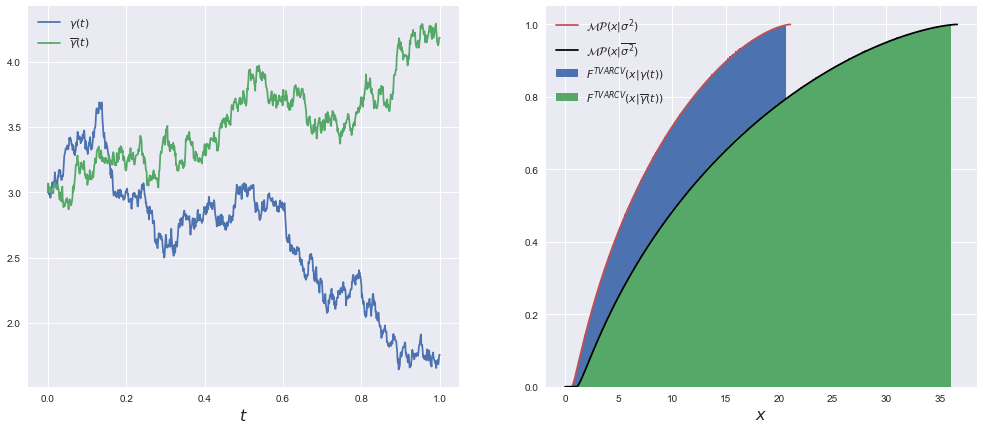
\includegraphics[scale=0.4]{XCIR}
    		\caption{$\eta_p = p, y = 0.5, \alpha = 5, \beta = 1, \gamma_0 = 3, \xi = 2$}
    		\smallskip
    		\small
    		Left panel shows two different realizations of $\gamma(t)$. On the right panel blue and green histograms are ESD of $\widehat{\Sigma}_p$ for corresponding volatility processes, red and black curve -- Marchenko-Pastur law for different realizations of $\sigma^2$. We see that even with the same parameters of volatility model, we have the different scale parameter in asymptotic spectral distribution for different realizations.
    	\end{center}
    \end{figure}
    
    \pagebreak
    \part{Jump-diffusion processes}
    \begin{rmrk}
    	(CHECK TEXT HERE!)
    	Before we discussed pure diffusion processes, namely that these processes are continuous almost sure. It is quite useful to consider so-called jump-diffusion processes... How should we change our estimator then?
    	ALSO MENTION ONE- AND FINITE-DIMENSIONAL PROCESSES, THEN GO FOR P->INF
    	ALSO WE ONLY CONSIDER EQUIDISTANT TIMES
    	AND ONLY SIGMA EQUAL TO IDENTITY, WHICH MEANS INDPENENCE
    	AND MU = 0
    \end{rmrk}
    
    \begin{exmp} \label{uniform jumps} \
    	\begin{enumerate}
    		\item Simplest model: let $U \sim \mathcal{U}[0, 1]$ be standard uniformly distributed random variable and
    		\begin{equation}
    		d\mathbf{X}(t) = \gamma(t)  d\mathbf{W}(t) + \Delta_U(t)dt,
    		\end{equation}
    		where $\Delta_U(t) = (\delta_U(t), \dots, \delta_U(t))^T$ is a vector of Dirac delta functions shifted to $U$. In other words, all the components of $\mathbf{X}(t)$ make a jump of size $1$ at the same random time $t = U$. Let us denote by $\mathbf{X^c}(t)$ the continuous part of $\mathbf{X}(t)$:
    		\[ d\mathbf{X^c}(t) = \gamma(t) d\mathbf{W}(t). \]
    		Moreover, let $\ell'$ denote the index of interval, where $U$ is located:
    		\[ U \in \bigg[\frac{\ell'-1}{n}, \frac{\ell'}{n}\bigg). \]
    		Then
    		\[ 
    		\begin{aligned}
    		\Sigma_p^{RCV} & = \sum_{\ell=1, \ell \neq \ell'}^{n}\Delta \mathbf{X}_\ell(\Delta \mathbf{X}_\ell)^T + \Delta \mathbf{X}_{\ell'}(\Delta \mathbf{X}_{\ell'})^T\\
    		& = \sum_{\ell=1, \ell \neq \ell'}^{n}\Delta \mathbf{X}_\ell(\Delta \mathbf{X}_\ell)^T + (\Delta \mathbf{X^c}_{\ell'} + \mathbb{U}_{p \times 1})(\Delta \mathbf{X^c}_{\ell'} + \mathbb{U}_{p \times 1})^T\\
    		& =  \sum_{\ell=1}^{n}\Delta \mathbf{X^c}_\ell(\Delta \mathbf{X^c}_\ell)^T + \Delta \mathbf{X^c}_{\ell'} \cdot \mathbb{U}_{1 \times p} + (\Delta \mathbf{X^c}_{\ell'} \cdot \mathbb{U}_{1 \times p})^T + \mathbb{U}_{p \times p} ,
    		\end{aligned}
    		\]
    		where $\mathbb{U}_{k \times j}$ stands for $k \times j$ matrix filled with ones. Note that the elements of $\Delta \mathbf{X^c}_{\ell'} \cdot \mathbb{U}_{1 \times p}$ are i.i.d. $ \sim \mathcal{N}\big(0, \Gamma_{\ell'}/n )$ with $\Gamma_{\ell'}=\int_{(\ell' - 1)/n}^{\ell' / n} \gamma^2(t) dt$. Therefore, if we set $n \rightarrow \infty$, $\tr(\Sigma_p^{RCV})$ will converge to the same value as before plus $p$. Also,
    		\[
    		\| \Delta \mathbf{X}_{\ell'} \|_2^2 = \| \Delta \mathbf{X^c}_{\ell'} + \mathbb{U}_{p \times 1} \|_2^2  = \sum_{j=1}^{p} (\Delta X^c_{\ell'})^2 + 2\sum_{j=1}^{p} \Delta X^c_{\ell'} + p.
    		\]
    		We have asymptotically:
    		\[
    		\sum_{j=1}^{p} (\Delta X^c_{\ell'})^2 \sim \frac{p}{n}\Gamma_{\ell'}
    		\]
    		as a sum of $p$ i.i.d. normally distributed random variables with variance $\Gamma_{\ell'}/n$ and
    		\[ \sum_{j=1}^{p} \Delta X^c_{\ell'} \sim \mathcal{N}\Big(0, \frac{p}{n}\Gamma_{\ell'}\Big). \]
    		As long as $p/n$ converges to some finite constant, $\Gamma_{\ell'}$ is bounded and $p$ converges to infinity, we have
    		\[ 
    		\frac{\Delta \mathbf{X}_{\ell'}(\Delta \mathbf{X}_{\ell'})^T}{\| \Delta \mathbf{X}_{\ell'} \|_2^2} \rightarrow 0.
    		\]
    		Hence, if we know that all components jumped at the same time and the size of the jump is equal to $1$, new estimator will be
    		\[ 
    		\widehat{\Sigma}_p = \frac{\tr(\Sigma_p^{RCV}) - p}{n} \sum_{\ell=1}^{n} \frac{\Delta \mathbf{X}_{\ell}(\Delta \mathbf{X}_{\ell})^T}{\| \Delta \mathbf{X}_{\ell} \|_2^2}.
    		\]
    		
    		\item Now let $U_1, \dots, U_p$ be i.i.d. $\sim \mathcal{U}[0, 1]$, $\mathbf{U} = (U_1, \dots, U_p)^T$ and
    		\[ 
    		d\mathbf{X}(t) = \gamma(t)  d\mathbf{W}(t) + \Delta_\mathbf{U}(t) dt
    		\]
    		with $\Delta_\mathbf{U}(t) = (\delta_{U_1}(t), \dots, \delta_{U_p}(t))^T$.
    	\end{enumerate}
    \end{exmp}
    
    \begin{rmrk}
    	In Example \ref{uniform jumps} we assumed that in the interval $[0, 1]$ each component of the process $\mathbf{X}(t)$ had exactly one jump. In practice, jump-diffusion processes are often modeled using Poisson processes, where one cannot be sure how many jumps can happen in given interval.
    \end{rmrk}
    
    \begin{defn} \
    	\begin{enumerate}
    		\item To construct a Poisson process, we begin with a sequence of arrival times $\tau_1^N, \tau_2^N, \dots$, where
    		\[ \tau_{j+1}^N - \tau_j^N \sim \operatorname{Exp}(\lambda) \quad \forall j \geq 1.  \]
    		This setting is similar to the one in Example \ref{PosTimes}, except that now $\tau_j^N$ stands for the time of $j$-th jump. \define{The Poisson process} $N(t)$ counts the number of jumps that occur at or before time $t$. More precisely,
    		\[ N(t) = \sum_{j \geq 1} \mathbf{1}_{ \{\tau_j^N \leq t\}}. \]
    		Because the expected time between jumps is $1/\lambda$, the jumps are arriving at an average rate of $\lambda$ per unit time. We say the Poisson process $N(t)$ has intensity $\lambda$.
    		\item Let $N(t)$ be a Poisson process with intensity $\lambda$, and let $Y_1, Y_2, \dots$ be a sequence of i.i.d. random variables with mean
    		\[ \beta = \ME[Y_1]. \]
    		We assume the random variables $Y_1, Y_2, \dots$ are also independent of $N(t)$. We define the \define{compound Poisson process}
    		\[ Q(t) = \sum_{i=1}^{N(t)} Y_i, \quad t \geq 0. \]
    		The jumps in $Q(t)$ occur at the same times as the jumps in $N(t)$, but whereas the jumps in $N(t)$ are always of size $1$, the $j$-th jump in $Q(t)$ is of random size $Y_j$.
    		\item A process $X(t)$ of the form
    		\[ X(t) = \int_{0}^t \mu(s)ds + \int_{0}^{t} \sigma(s) dW(s) + J(t), \]
    		where $\mu(s), \sigma(s)$ are adapted processes, $W(s)$ is a standard Brownian motion and $J(t)$ is an adapted right-continuous pure jump process with $J(0) = 0$, is called a \define{jump-diffusion process}.
    	\end{enumerate}
    \end{defn}
    
    \begin{prps}
    	Let $X_1(t) = \int_{0}^t \mu_1(s)ds + \int_{0}^{t} \sigma_1(s) dW(s) + J_1(t)$ be a jump-diffusion process. Then
    	\[ [X_1, X_1](t) = \int_0^t \sigma_1^2(s)ds + \sum_{0 < s \leq t} (\Delta J_1(s) )^2. \]
    	Let also $X_2(t) = \int_{0}^t \mu_2(s)ds + \int_{0}^{t} \sigma_2(s) dW(s) + J_2(t)$, then
    	\[ [X_1, X_2](t) = \int_0^t \sigma_1(s) \sigma_2(s) ds + \sum_{0 < s \leq t} \Delta J_1(s)\Delta J_2(s). \]
    \end{prps}
    \begin{proof}
    	See Theorem 11.4.7 in Shreve
    \end{proof}
    
    \begin{rmrk}
    	Let us again look at the case with fixed $p$. IF WE HAVE U1, THEN WE HAVE
    	\[ \Sigma_p^{RCV} \xrightarrow{\MP} \Sigma_p + \mathbb{U}_{p \times p}  \]
    	OR IN THE CASE OF U2:
    	\[ \Sigma_p^{RCV} \xrightarrow{\MP} \Sigma_p + \mathbb{I}_{p \times p}  \]
    	(CHECK IT IN SIMULATIONS)
    	BUT WHAT IF P IS INFINITE?
    \end{rmrk}
    
    \pagebreak
    \part{Simulation studies}
    \section*{Non-constant volatility}
    
    \begin{rmrk}
    	BLA BLA BLA Here we do simulations
    \end{rmrk}
    
    \begin{exmp} \label{SimCos}
    	Let's take an example from the paper...
    	\[
    	\gamma(t) = \sqrt{0.0009 + 0.0008 \cos(2 \pi t)}.
    	\]
    	Then
    	\[ \sigma^2 = 0.0009 + \int_{0}^{1}0.0008 \cos(2 \pi t) dt = 0.0009. \]
    	The simulations show that TVARCV estimator converges asymptotically to Marchenko-Pastur law, while RCV converges to ???
    \end{exmp}
    
    
    \section*{Non-equidistant observation times}
    \begin{figure}
    	\begin{center} \centering
    		\includegraphics[scale=0.4]{XCos2}
    		\caption{ $\mathbf{X}(t)$ from Example \ref{SimCos}, $n = 1000$, $p=4000$, $\sigma^2 = 0.0009$ }
    		\smallskip
    		\small
    		In this setting $y = p/n = 4$. One the left panel one sees four thousands independent stochastic processes. On the right blue histogram shows ESD of $\Sigma_p^{RCV}$, green histogram -- ESD of $\widehat{\Sigma}_p$ and red curve -- Marchenko-Pastur law. Note point mass equal to $0.75$ at the origin.
    	\end{center}
    \end{figure}
    
    \begin{exmp} \label{PosTimes}
    	Let us set time points $ \{\tau_\ell\}_{0 \leq \ell \leq n}$, where $\tau_0 = 0$ a.s. and interarrival times are independent and obey the exponential distribution with rate $\lambda$, that is 
    	\[ \MP(\tau_{\ell} - \tau_{\ell-1} > x) =  e^{-\lambda x}, \quad 1 \leq \ell \leq n. \]
    	Then by Strong Law of Large Numbers
    	\[ \frac{\tau_n}{n} = \frac{1}{n} \sum_{\ell=1}^{n} (\tau_{\ell} - \tau_{\ell-1}) \xrightarrow{a.s.} \ME[\tau_1] = \lambda. \]
    	Define
    	\[ \mathcal{T} = \{\tau_\ell : \tau_\ell \in [0, 1]\}, \]
    	then by setting $\lambda = \frac{1}{n}$, we get $\#\mathcal{T} \sim n$.
    	Let's take volatility $\gamma_t$ as in Example \ref{SimCos}.
    	(CONSIDER WHEN TAU DEPENDS ON X, SO THE LAST ASSUMPTION WON'T BE SATISFIED)
    \end{exmp}
    
    \begin{figure}
    	\begin{center} \centering
    		\includegraphics[scale=0.4]{XCos}
    		\caption{ $\mathbf{X}(t)$ from Example \ref{SimCos}, $n = 1000$, $p=1000$ }
    		\smallskip
    		\small
    		In this setting $y = p/n = 1$. Note, that the domain of $F^{RCV}$ is larger than the domain of Marchenko-Pastur law, as it was proved in Proposition \ref{counter RCV}.
    	\end{center}
    \end{figure}
    
    \begin{figure}
    	\begin{center} \centering
    		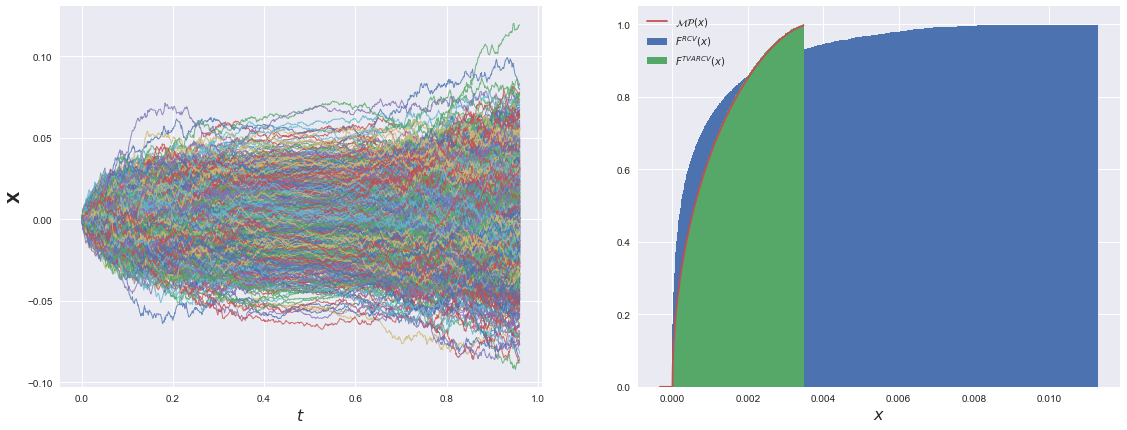
\includegraphics[scale=0.4]{Xcostimes}
    		\caption{ $\mathbf{X}(t)$ from Example \ref{PosTimes}, $n \simeq 1000$, $p=1000$ }
    		\smallskip
    		\small
    		We see that if observation times are not equidistant, the ESD of RCV changes drastically, even if visually there is no difference in realizations of $\mathbf{X}(t)$ and volatility process $\gamma(t)$ stays the same.
    	\end{center}
    \end{figure}
    
    \section*{INTERESTING CASE}
    \begin{rmrk}
    	For TVARCV to converge to Marchenko-Pastur law, it is sufficient, but not necessary, that $\mathbf{X}(t)$ belongs to  the class $\mathcal{C}$. Morevover, we can show that it might be the case when we have convergence even for RCV.
    \end{rmrk}
    \begin{exmp} \label{counter exmpl}
    	Let as usual $\boldsymbol{\mu}(t) =0$ and $\Theta(t)$ be diagonal matrix, defined as follows:
    	\[ \Big(\Theta(t)\Big)_{jj} = \cos(\pi t) \mathbf{1}_{\{j \leq p/2\}} + \sin(\pi t) \mathbf{1}_{\{j > p/2\}}, \quad 1 \leq j \leq p.  \]
    	In other words, first $p/2$ elements of the diagonal of $\Theta(t)$ are $\cos(\pi t)$ and the others are $\sin(\pi t)$. It is clear, that $\mathbf{X}(t)$ doesn't belong to thr class $\mathcal{C}$. The ICV matrix is in this case
    	\[ \Sigma_p = \begin{pmatrix}
    	\int_{0}^{1} \cos(\pi t)^2 dt & \cdots & 0 \\
    	\vdots & \ddots & \vdots \\
    	0 & \cdots & \int_{0}^{1} \sin(\pi t)^2 dt
    	\end{pmatrix} 
    	= \frac{1}{2} \mathbb{I}_{p \times p}. \]
    \end{exmp}
    
    \begin{figure}
    	\begin{center} \centering
    		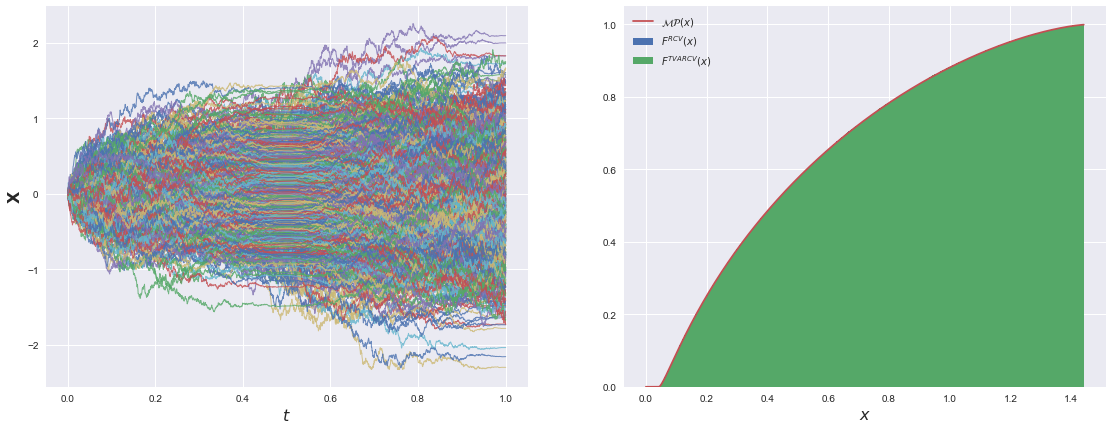
\includegraphics[scale=0.4]{counter}
    		\caption{ $\mathbf{X}(t)$ from Example \ref{counter exmpl}, $n = 3000$, $p=1000$ }
    		\smallskip
    		\small
    		Blue and green histograms coincide...
    	\end{center}
    \end{figure}
    
    \begin{exmp}
    	Let us change slightly the structure of $\Theta(t)$:
    	\[ \Big(\Theta(t)\Big)_{jj} = \cos(\pi t) \mathbf{1}_{\{j \leq p/4\}} + \sin(\pi t) \mathbf{1}_{\{j > p/4\}}, \quad 1 \leq j \leq p.\]
    	The ICV matrix $\Sigma_p$ stays the same. But we see that both estimators RCV and TVARCV are not converging to Marchenko-Pastur law anymore.
    \end{exmp}
    
    \pagebreak
    \part{Conclusion}
    
    \pagebreak
    \begin{appendices}
    	\part*{Cumulative distribution for Marchenko-Pastur law}
    	
    	\pagebreak
    	\part*{Python code}
    	\begin{python}
import seaborn as sns
import matplotlib.pyplot as plt
import matplotlib
import numpy as np  
  		
    		
# Marchenko-Pastur probability density function
def MPPdf(x, y, sigmaSq):
    if x == 0:
        if y > 1:
            return np.inf
        return 0
    sqrtY = np.sqrt(y)
    a = sigmaSq * (1 - sqrtY) * (1 - sqrtY)
    b = sigmaSq * (1 + sqrtY) * (1 + sqrtY)
    if x < a or x > b:
        return 0
    pdf = np.sqrt((b - x) * (x - a))
    pdf /= (y * x)
    pdf /= (2 * np.pi * sigmaSq)
    return pdf


# Marchenko-Pastur cumulative distribution function
def MPCdf(x, y, sigmaSq):
    # Marchenko-Pastur cdf for y > 1
    def MPCdfLargeRatio(x, y):
        y1 = 1 - x + y
        temp = np.sqrt(4 * y - y1 * y1)
        y1 /= temp
        y1 = (1 + y) * np.arctan(y1)
        y2 = x * (1 + y)
        y2 -= (y - 1) * (y - 1)
        y2 /= (temp * (y - 1))
        y2 = (y - 1) * np.arctan(y2)
        cdf = np.pi - temp + y1 + y2
        cdf /= (2 * np.pi * y)
        return 1 - cdf

    # Marchenko-Pastur cdf for y <= 1
    def MPCdfSmallRatio(x, y):
        y1 = 1 - x + y
        temp = np.sqrt(4 * y - y1 * y1)
        y1 /= temp
        y1 = (1 + y) * np.arctan(y1)
        if y == 1:
            y2 = 0
        else:
            y2 = x * (1 + y)
            y2 -= (y - 1) * (y - 1)
            y2 /= (temp * (1 - y))
            y2 = (y - 1) * np.arctan(y2)
        cdf = np.pi * y + temp - y1 + y2
        cdf /= (2 * np.pi * y)
        return cdf

    x0 = x / sigmaSq
    sqrtY = np.sqrt(y)
    a = (1 - sqrtY) * (1 - sqrtY)
    b = (1 + sqrtY) * (1 + sqrtY)
    if x0 >= b:
        return 1
    if x0 < 0:
        return 0
    if y > 1:
        if x0 <= a:
            return 1 - 1 / y
        return MPCdfLargeRatio(x0, y)
    if x0 <= a:
        return 0
    return MPCdfSmallRatio(x0, y)


# get sorted eigenvalues
def get_sorted_eigvals(Sigma):
    return np.sort(np.linalg.eigvals(Sigma))


# get empirical spectral distribution
def ESD(x, sorted_eig_values):
    numerator = len(sorted_eig_values[sorted_eig_values <= x])
    denominator = len(sorted_eig_values)
    return numerator / denominator


# TVARCV
def TVARCV(dX, Sigma_RCV):
    (p, n) = dX.shape
    Sigma = np.zeros((p, p))
    minnorm = p
    maxnorm = 0
    for l in range(n):
        dX_l = np.matrix(dX[:, l]).transpose()
        norm = np.linalg.norm(dX_l, ord=2)
        Sigma += dX_l.dot(np.transpose(dX_l)) / (norm * norm)
    Sigma *= np.trace(Sigma_RCV) / n
    return Sigma


# RCV
def RCV(dX):
    (p, n) = dX.shape
    Sigma = np.zeros((p, p))
    for l in range(n):
        dX_l = np.matrix(dX[:, l]).transpose()
        Sigma += dX_l.dot(np.transpose(dX_l))
    return Sigma
  

# function to plot stochastic processes in Figure 1
def plot_exmp_1():
    n = 10000
    time = np.linspace(0, 1, n)
    mu = np.array([0, 0, 0])
    X = np.zeros((n, 3))
    dt = time[1] - time[0]
    sqrt_dt = np.sqrt(dt)
    dX = np.random.normal(0, sqrt_dt, 3)
    X[1] = X[0] + dX
    for i in range(1, n - 1):
        dW = np.random.normal(0, sqrt_dt, 3)
        Theta = np.identity(3)
        Theta[0][1] = Theta[1][0] = np.cos(np.pi * time[i])
        Theta[0][2] = Theta[2][0] = np.sin(np.pi * time[i])
        dX_l = np.dot(Theta, dW)
        dX_l += mu * dt
        X[i + 1] = X[i] + dX_l
        dX = np.c_[dX, dX_l]

    plt.plot(time, X)
    plt.legend(["$X_1(t)$", "$X_2(t)$", "$X_3(t)$"], fontsize = 16)
    plt.xlabel('$t$', fontsize = 16)
    plt.ylabel('$\mathbf{X}$', fontsize = 16)
    plt.show()


# function to plot graphs of Marchenko-Pastur law (Figure 2)
def plot_MP_law
    y = [0.1, 0.25, 1, 4]
    sigma_sq = [1, 1, 1, 0.3]
    m = 300
    xpdf = np.linspace(1/m, 4, m)
    xcdf = np.linspace(-1/m, 4, m)
    cdf = np.zeros(m)
    pdf = np.zeros(m)
	
    plt.subplot(1, 2, 1)
    for ratio, vol in zip(y, sigma_sq):
        for i in range(m):
    	    pdf[i] = MPPdf(xpdf[i], ratio, vol)
        plt.plot(xpdf, pdf)
    plt.ylim(ymax=2.25)
    # plot infinity line for y > 1
    plt.plot((0, 0), (0, 3), color='C3')
    plt.legend(["$y=0.1, \sigma^2=1$", "$y=0.25, \sigma^2=1$", \
        "$y=1, \sigma^2=1$", "$y=4, \sigma^2=0.3$"])
    plt.xlabel('$x$', fontsize = 16)
    plt.ylabel('$f(x)$', fontsize = 16)
	
    plt.subplot(1, 2, 2)
    for ratio, vol in zip(y, sigma_sq):
        for i in range(m):
            cdf[i] = MPCdf(xcdf[i], ratio, vol)
        plt.plot(xcdf, cdf)
    plt.legend(["$y=0.1, \sigma^2=1$", "$y=0.25, \sigma^2=1$", \
        "$y=1, \sigma^2=1$", "$y=4, \sigma^2=0.3$"]) 
    plt.xlabel('$x$', fontsize = 16)
    plt.ylabel('$F(x)$', fontsize = 16)
	
    plt.show()
    	\end{python}
    	
    \end{appendices}
\end{document}
